% Template for a Computer Science Tripos Part II project dissertation
\documentclass[12pt,a4paper,twoside,openright]{report}
\usepackage[pdfborder={0 0 0}, breaklinks]{hyperref}    % turns references into hyperlinks
\usepackage[margin=25mm]{geometry}  % adjusts page layout
\usepackage{graphicx}  % allows inclusion of PDF, PNG and JPG images
\usepackage{docmute}   % only needed to allow inclusion of proposal.tex
\usepackage{listings}
\usepackage{tikz}
\usepackage{adjustbox}
\usepackage{multirow}

% tikz settings
\usetikzlibrary{shapes, arrows, positioning}

\raggedbottom                           % try to avoid widows and orphans
\sloppy
\clubpenalty1000%
\widowpenalty1000%

\renewcommand{\baselinestretch}{1.1}    % adjust line spacing to make
                                        % more readable

\definecolor{keywords}{RGB}{220,0,90}
\definecolor{strings}{RGB}{0,140,0}
\definecolor{comments}{RGB}{0,127,0}
\definecolor{identifiers}{RGB}{20,20,75}

\lstset{basicstyle=\ttfamily\small,
    basewidth={.5em, .3em},
    keywordstyle=\color{keywords},
    commentstyle=\color{comments},
    stringstyle=\color{strings},
    showstringspaces=false,
    % identifierstyle=\color{identifiers},
    escapechar=$ %$
    }

\newcommand{\cbox}[2]{\adjustbox{bgcolor=#1}{#2}}

\begin{document}

\bibliographystyle{plain}


%%%%%%%%%%%%%%%%%%%%%%%%%%%%%%%%%%%%%%%%%%%%%%%%%%%%%%%%%%%%%%%%%%%%%%%%
% Title


\pagestyle{empty}

\rightline{\LARGE \textbf{Tianlin Zhang}}

\vspace*{60mm}
\begin{center}
\Huge
\textbf{An Observable OCaml} \\[5mm]
Computer Science Tripos -- Part II \\[5mm]
Jesus College \\[5mm]
\today  % today's date
\end{center}

%%%%%%%%%%%%%%%%%%%%%%%%%%%%%%%%%%%%%%%%%%%%%%%%%%%%%%%%%%%%%%%%%%%%%%%%%%%%%%
% Proforma, table of contents and list of figures

\pagestyle{plain}

\chapter*{Proforma}

{\large
\begin{tabular}{ll}
Name:               & \bf Tianlin Zhang \\
College:            & \bf Jesus College\\
Project Title:      & \bf An Observable OCaml\\
Examination:        & \bf Computer Science Tripos -- Part II\\
Year:               & \bf June 2018\\
Word Count:         & \bf 11981\footnotemark \\
Project Originator: & Stephen Kell \\
Supervisor:         & Stephen Kell \\ 
\end{tabular}
}
\footnotetext{This total computed with \texttt{pdftotext
        tz286\char`_dissertation1.pdf - | wc -w}.}

\section*{Original Aims of the Project}

To write a backend for the OCaml compiler that allows compilation from OCaml 
into C in such a way that it preserves so-called ``observability'', that is the 
ability to debug the generated C code, using GDB for example, in a similar 
fashion to debugging the original OCaml code. A library of test programs should 
be written to demonstrate the capabilities of the compiler, along with an 
evaluation into the performance and observability of the compiled code.

\section*{Work Completed}

I have written and completed a new backend for the OCaml compiler which can
compile a suitable target subset of OCaml, including a majority of the most
commonly used features. A C runtime library has also been written to support the
execution of the resulting C output, as well as a library of test programs which
are used in testing and evaluation of the compiler. An evaluation has also been
performed investigating the execution times of the compiler with respect to the
OCaml native compiler, and the observability of the compiled code with the OCaml
bytecode compiler.

\section*{Special Difficulties}

None.
 
\newpage
\section*{Declaration}

I, Tianlin Zhang of Jesus College, being a candidate for Part II of the Computer
Science Tripos, hereby declare
that this dissertation and the work described in it are my own work,
unaided except as may be specified below, and that the dissertation
does not contain material that has already been used to any substantial
extent for a comparable purpose.

\bigskip
\leftline{Signed: Tianlin Zhang}

\medskip
\leftline{Date: \today}

\tableofcontents

%%%%%%%%%%%%%%%%%%%%%%%%%%%%%%%%%%%%%%%%%%%%%%%%%%%%%%%%%%%%%%%%%%%%%%%
% now for the chapters

\pagestyle{headings}

\chapter{Introduction}

My project concerns the creation of a new compiler for OCaml, a popular
statically typed functional language in the ML family, into the C language in
such a way as to be able to take advantage of debugging tools provided by the C
toolchain. This property, henceforth referred to as ``observability'', refers to
the ability to view the execution of the program through a debugger as if it was
debugging a C program and to recover the program's execution state.

I have successfully implemented a compiler for a core subset of the OCaml
language in to C, which when compiled with a standard C compiler such as
\texttt{gcc} or \texttt{clang} produces an executable that behaves in an
identical way up to minor differences with the output of the native OCaml
compiler. Additionally, when compiled with the \texttt{-g} flag, the resulting
executable can be debugged under \texttt{gdb} in such a way that preserves the
execution order of the original OCaml source, and allows setting breakpoints and
observing values in the OCaml code in the same way as if it were debugging the
original OCaml code.

In addition, the compiler performs well in comparison with both the OCaml native
compiler and the bytecode compiler, creating executables that execute with
similar speeds to the native compiler and debug in a similar manner to the OCaml
debugger.

\section{Motivation}

There are several motivations for this project, including:

\subsubsection{Observability}

The OCaml debugger was introduced fairly recently, and only works on compiled 
bytecode; in addition, since OCaml strips away type information on actual 
values at runtime, the debugger is unable to inspect the values of certain 
variables within polymorphic functions.

We can consider the following example OCaml code:

\begin{lstlisting}[language=Caml]
let id x = x
let a = id 2
\end{lstlisting}

Running this through the OCaml debugger, we see that it is unable to determine
the value of the variable \texttt{x} within the \texttt{id} function.

\begin{lstlisting}
(ocd) break @ Id 1
Breakpoint 1 at 10156: file id.ml, line 1, characters 12-13
(ocd) run
Time: 12 - pc: 10156 - module Id
Breakpoint: 1
1 let id x = <|b|>x
(ocd) print x
x: 'a = <poly>
\end{lstlisting}

Compiling to C could take advantage of a different data representation, and GDB
extensions to customise debugger behaviour, allowing GDB to `see-through'
polymorphic values such as this..

\subsubsection{Plausibility} There are many language features in OCaml which do
not have similar analogues in C. Examples of these include algebraic data
structures, partial application, lexical closures, and polymorphic datatypes and
functions. I was interested in whether despite these differences, I could create
appropriate transformations to simulate these in C but preserve observability at
the same time, giving an OCaml view into what the code is doing.

\subsubsection{Performance}

By compilation to C, I can take advantage of the fact that the most popular C 
compilers have undergone decades of optimisation to produce very performant 
code. We can exploit this to obtain very fast executables without needing to 
perform much optimisation on the OCaml code. There will however be performance 
trade-offs in terms of emulating OCaml function calls in C compared to normal 
function calls, as OCaml functions can take advantage of features such as
lexical closures and partial application, as well as being first-class allowing
them to be passed as values to higher-order functions.

\section{Previous Work}

There exist prior work for compiling ML-like languages into C
\cite{noassemblyrequired} but the approach used is to transform the program into
continuation-passing style. This is not suitable for the compiler as it would
interfere with the program execution and make it untenable to map OCaml source
code into regions of the compiled code for debugging purposes, but shows that
compilation into C from similar functional languages is feasible.

In addition, this project was also attempted in previous years by a previous
student \cite{previousproject} under the same supervisor with a similar starting
point, but my approach to the design of the compiler was not influenced and it
is of my opinion that a sufficiently different approach was used for this
project. A different representation of the output C code was used leading to a
different compiler structure from the outset of the project, as well as
completely different approaches being taken for more complex features in OCaml,
such as data representation and closure conversion.

\chapter{Preparation}

Before starting the project I had significant experience with functional
languages through the Standard ML course undertaken and also personal experience
with programming in Haskell, but I had never used OCaml at length, nor worked
with the OCaml compiler codebase. While OCaml was very simple to learn from my
previous experiences with functional languages, the OCaml compiler codebase was
large, complex, and very sparsely commented.

In this respect, a large portion of time during the starting weeks of the 
project was focused on reading through barely-commented source code in order to
understand the different data types used by the OCaml compiler, as well as
research into various options for different libraries to use.

\section{Starting point}

The starting point of this project is the existing OCaml
compiler\footnote{\url{https://github.com/ocaml/ocaml}}, as it would be too
onerous to duplicate the effort of parsing and performing type inference on
OCaml source code. Instead, my compiler takes the \texttt{Lambda} intermediate
representation from the OCaml compiler and compiles this into C. Since the OCaml
compiler backends Asmgen and Bytegen, which produce the native binaries/bytecode
executables, also only take the \texttt{Lambda} IR, this approach is akin to
introducing a new compiler backend or different target for compilation.

\begin{figure}
    \centering
    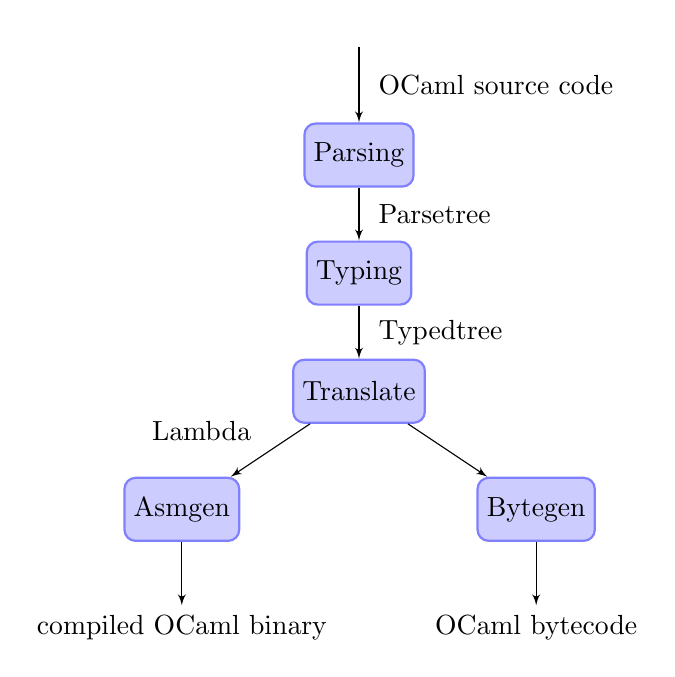
\begin{tikzpicture}[
blank/.style={node distance=1.5cm},
block/.style={rectangle, text centered, rounded corners, minimum height=0.8cm, 
node distance=1.5cm, thick, draw=blue!50, fill=blue!20},
block-emph/.style={block, draw=red!50, fill=red!20},
block-neutral/.style={block, draw=black!50, fill=black!20},
line/.style={draw, -latex'}
]
\node [blank] (start) {};
\node [block, below of=start] (parsing) {Parsing};
\node [block, below of=parsing] (typing) {Typing};
\node [block, below of=typing] (translate) {Translate};
\node [block, below of=translate, xshift=2.25cm] (bytegen) {Bytegen};
\node [blank, below of=bytegen] (compiled-byte) {OCaml bytecode};
\node [block, below of=translate, xshift=-2.25cm] (asmgen) {Asmgen};
\node [blank, below of=asmgen] (compiled-asm) {compiled OCaml binary};

\path [line] (start) -- node [midway, label=right:{OCaml source code}] {}
(parsing);
\path [line] (parsing) -- node [label=right:{Parsetree}] {} (typing);
\path [line] (typing) -- node [label=right:{Typedtree}] {} (translate);
\path [line] (translate) -- node [label=left:{Lambda}, yshift=0.25cm] {} (asmgen);
\path [line] (asmgen) -- (compiled-asm);
\path [line] (translate) -- (bytegen);
\path [line] (bytegen) -- (compiled-byte);
\end{tikzpicture}
    \caption{A representation of the various stages in the OCaml compiler. 
    Adapted from \cite[Chapter~22]{realworldocaml}.}
    \label{fig:compilerstages}
\end{figure}

The rest of this section will address why this was chosen as the starting 
point, and the process during the preparation phase in which the appropriate 
starting point was determined.

\subsection{Intermediate representations}

The OCaml compiler processes code in the pipeline shown in
figure~\ref{fig:compilerstages}, with the pipeline branching towards the end
into two separate stages representing the targets that the OCaml compiler can
compile to. Between each stage, a different intermediate representation of the
code is produced.

One of the tasks that had to be carried out during the preparation phase was 
to determine which intermediate representation would be most suitable for 
compilation into C. The requirements required for such an intermediate 
representation would be:

\begin{itemize}

\item It must be easy to recover type information from the representation. This
    is because the resulting C code must be statically typed also, so we need to
    be able to infer the types of variables and functions in order for them to
    be implemented in C.

\item The representation must be fairly normalised, with as few as possible
    language constructs to simplify the translation into C. Many language
    features in OCaml are merely syntactically sugared versions of more
    primitive ones (for example, pattern matching is really a combination of
    branching based on the value of a variable plus some variable bindings for
    unpacking) which must have been desugared anyway during the compilation
    process, so it would be more useful if we could utilise an intermediate
    representation for which this has already happened.

\item The representation must also allow some amount of reconstruction back to
    the source level, so we can map the output code to the correct sections of
    the source code. This is important for observability and debugging as we
    would like debuggers to display the correct segments of code being debugged.
    This does however present an antagonism, where we would like the IR to be
    both normalised, but not enough that we cannot recover any source-level
    information from it.

\end{itemize}

\subsubsection{\texttt{Parsetree}}

\texttt{Parsetree} is a parsed AST representation of the source code, which 
essentially directly represents the original OCaml source code. No processing 
has occurred on any language constructs, and type inference has not even 
occurred on the IR. This obviously makes this intermediate representation 
unsuitable as the choice of IR, since it falls down on both ability to recover 
type information and normalisation.

\subsubsection{\texttt{Typedtree}}

\texttt{Typedtree} is a type-annotated AST which is almost exactly identical to 
the \texttt{Parsetree} IR, except that expressions have been annotated with a 
type. This makes this IR highly desirable as the starting point for compilation 
into C, and was initially where the investigation for a usable intermediate 
representation started.

However, since \texttt{Typedtree} still almost directly represents the original
source code, it suffers from the same normalisation problem as
\texttt{Parsetree} does. For example, the number of different sub-expression
cases that \texttt{Parsetree} represents separately is 31 --- modules, classes
and objects are still represented as syntactical elements; records, variants,
and field accesses have not been normalised into one representation; and pattern
matches have not been simplified but instead stored as association lists of raw
patterns to expressions.

This makes the \texttt{Typedtree} IR very cumbersome to work with, and 
ultimately it was considered unsuitable for the starting point of the project.

\subsection{The \texttt{Lambda} IR}

The \texttt{Lambda} IR is so named because it resembles an untyped lambda 
calculus, and is what in fact the two existing backends of the compiler 
generate code from. It has a number of advantages over \texttt{Parsetree} and 
\texttt{Typedtree}, including:

\begin{itemize}

\item Variants and records have been normalised into one representation, which
    is referred to as a block, which are similar to tagged unions. In addition,
    variants without parameters are compiled into bare integers.

\item Desugaring of pattern match statements. Because variants have been
    compiled into integers or tagged unions, the translation pass is able to
    optimise pattern matching into switch statements. In very simple cases,
    pattern matches are in fact compiled into an if-else statement instead.

\item Removal of modules and functors. These values have instead been compiled
    into equivalent representations using blocks and functions.

\end{itemize}

In comparison to \texttt{Typedtree}'s 31 different cases for sub-expressions, 
the \texttt{Lambda} representation has 20 different cases, which are relatively 
much simpler than those in \texttt{Typedtree}. This makes the \texttt{Lambda} 
IR far more desirable as a starting point.

However, there are some major disadvantages of the \texttt{Lambda} IR:

\begin{itemize}

\item The translation pass into \texttt{Lambda} does not preserve much of the
    type information from \texttt{Typedtree}. This is a huge problem which is
    solved somewhat with the existence of \texttt{Lambda} events, which will be
    discussed in \S\ref{lambda-types}.

\item Normalisation in the \texttt{Lambda} IR discards a lot of source-level
    information such as which source-level expressions \texttt{Lambda}
    expressions map to, as well as having very little information about the
    location in the source code of the current code. This is somewhat remedied
    with \texttt{Lambda} events, which is discussed in \S\ref{line-directive}.

\item The \texttt{Lambda} IR has not yet had closure conversion applied to it.
    Functions are still represented in a similar fashion to how they were in the
    original source code, meaning the cases of lexical closures, partial
    application, etc. are not handled.

\end{itemize}

It was determined that while the \texttt{Lambda} IR does not fully satisfy the
typing and source reconstruction requirements, enough type and source
information was recoverable that it was deemed acceptable as a starting point.
Thus, my project starts compilation by obtaining the \texttt{Lambda}
representation by passing the source code through part of the compilation
pipeline, and then translates the resulting IR into C from that point onwards.

\section{Extensibility of GDB}

Part of the project requirements dictate that the resulting code be 
``observable'', and it was quickly identified that if GDB is to be used as the 
primary debugger it may be necessary to extend GDB in order to handle the 
compiled OCaml code correctly and display recursive OCaml values. Thus, a brief 
investigation into GDB was carried out in the preparation phase to investigate 
its extensibility.

One of the experiments which was carried out was to see if GDB could display
code from other files, and associate parts of compiled C code with instead parts
of code from another file. This is a necessary part of the compilation process,
as the resulting debuggable executable must display code and symbols from the
original OCaml file from which it was compiled from via my compiler, not the C
file that my compiler produces. With some investigation it was found that this
was possible with the \texttt{\#}\texttt{line} directive, which is explored in
\S\ref{line-directive}.

Another feature which is required for observability is the ability to display 
OCaml values at least recursively, if not formatted in the same way as the 
OCaml compiler does. This is because many OCaml values are recursive (for 
example, the list type is a recursive type which refers back to itself as one 
of its parameters) so it must be possible to extend GDB with some way to 
recursively print values whenever it finds a pointer. It was found that GDB 
does support extensions to itself via custom macros, and also supports custom 
pretty-printers (via, for example, Python) for different types. Either of these 
features would allow GDB to display OCaml values correctly.

\section{Target subsets}

During the write-up of the project proposal, three expanding subsets of OCaml 
were identified in order to structure the creation of the compiler around. 
These subsets represent a grouping of similar constructs and features together 
such that each subset focuses on a similar theme in the new features it 
introduces.

Identification of these subsets firstly has the benefit of providing a clear 
structure to the project, and greatly influenced the order in which features 
were implemented. Optimistically, it was expected that at the end of proposed 
deadlines a compiler would be completed that could compile the associated 
Subset -- unfortunately, due to interdependence between a lot of the features a 
working compiler was not produced until towards the end of implementing 
features for Subset 2.

These subsets also serve to identify what the minimum viable product of the 
project is, as it was determined on project conception compilation of the 
entire OCaml language would be far too ambitious. As such, Subset 3 represents 
the subset of the language that the final product should at minimum be able to 
compile correctly.

Despite the fact that the subsets ultimately did not produce distinct and 
recognisable milestones for compilers that could operate on the appropriate 
subsets of the language, it is still worth describing the subsets for the 
effect they had on the planning for the rest of the project.

\subsection{Subset 1}

Subset 1 is a very simple language with only a limited number of types and 
language constructs. This subset contains only basic boolean, integer, floating 
point, and \texttt{unit} types, only basic string support (for input/output), 
top level function declarations with \texttt{let} and \texttt{let rec}, and 
basic language constructs such as \texttt{if}, \texttt{for}, and \texttt{while}.

\subsection{Subset 2}

Subset 2 expands on Subset 1 by introducing custom types and polymorphism. This 
includes tuples, lists, variant types via algebraic data types, record types, 
match expressions and function parametric polymorphism. This subset is aimed 
towards designing and implementing an appropriate representation of OCaml 
values in C, as well as a way of representing polymorphic values both as values 
in user-defined types and as parameters to functions.

\subsection{Subset 3}

Subset 3 expands further on Subset 2 by adding treatment of functions as first
class values, plus closure conversion features, which would entail compilation
of lexical closures, partial application, anonymous functions, etc. The focus of
this subset is intended towards the design and implementation of closures in C,
and correctly compiling the more difficult features of OCaml functions into C.

\section{The \texttt{liballocs} library}

\texttt{liballocs}\cite{liballocs} is a library that is able to track all
allocations in memory and their associated types with no extra required effort.
It exposes an interface that, when given an arbitrary pointer, is able to return
information about the type of the value in the allocated memory. This was
identified to be extremely useful for implementing observability features, as it
could be used within polymorphic functions to determine the type of certain
values whilst debugging at runtime, which would be an advantage over the OCaml
bytecode debugger, which due to the untagged nature of OCaml values cannot
determine the type of polymorphic values at runtime.

Unfortunately, it was deemed that explicit tagging of types was easier to
implement than inclusion of the \texttt{liballocs} library, but future
extensions to the compiler may incorporate it to provide more detailed typing
information.

\section{The Boehm GC}

Since the target subset aims to include a significant portion of OCaml including
parts which allow for data structures and closures to be created. It is
necessary that the runtime would require some sort of garbage collection. For
reference, the OCaml native compiler includes as part of its runtime a
specialised garbage collector written specifically for OCaml programs.

Writing a new garbage collector would be very complex and heavily outside the
scope of the project, so we would like to make use of a pre-existing solution
for garbage collection in C. Fortunately, many garbage collectors exist, and the
Boehm GC\footnote{\url{http://www.hboehm.info/gc/}} was selected and used.

The Boehm GC is a garbage collector for C and C++, which exposes a function
\texttt{GC\char`_MALLOC} which can works as a replacement for \texttt{malloc}.
Whenever \texttt{GC\char`_MALLOC} is called, it runs the garbage collector by
scanning the stack for values that could potentially look like pointers and so
performing garbage collection. This means that in simple cases, it can be used
as a drop-in solution for GC without extra configuration.

\section{Setting up the environment}

The source code of the compiler was managed using \texttt{git}, the repository
of which was backed up by publishing to
GitHub\footnote{\url{https://github.com/t-veor/observable-ocaml}}. Development
initially took place on the master branch, but once the compiler approached
feature completeness new features in the compiler would be developed in a forked
branch, worked on until they pass the regression tests, and then merged into the
master branch.

In addition, a copy of the source code was continuously backed up using Dropbox,
which was synced between two local copies of the code, on two separate machines.
In this manner, the code had four points of redundancy in the case of any
computer failures.

\section{Licensing of external code}

The principal body of code being used is the OCaml core
system\footnote{\url{https://github.com/ocaml/ocaml/blob/4.05/LICENSE}}, which
is released under LGPL v2.1. LGPL is a more permissive version of the GPL
license, intended for use for libraries rather than full pieces of software. The
LGPL license puts restrictions on what it calls ``derivative works of the
Library'', which are either modifications of the library or other software that
includes the library or statically link to it, requiring that these derivative
works are open source and also released with either the LGPL or the GPL library.

However, software that is designed to work with the library by linking against
it but does not actually contain any portion of the library fall outside the
scope of the license, which is the case with my compiler. As I am only releasing
the source code of the compiler, which do not contain parts of the OCaml core
system but link against it, the LGPL terms do not apply to the source code. They
would however apply if I decided to release a compiled executable which has
statically linked in the OCaml core system, but in fact a special exemption in
the OCaml's core system also covers this, allowing works which statically or
dynamically link with a publicly distributed version of the OCaml core system
to be exempt from the clauses of LGPL.

The other main library used is the Boehm
GC\footnote{\url{http://www.hboehm.info/gc/license.txt}}, which uses a custom
permissive free software license, allowing for distribution and modification as
long as a copy of the license is distributed with the library. This means in
fact that my code is not within the scope of the license, since I do not
distribute any part of the Boehm GC, but merely link against it in the
compilation process. I have included the license within my repository
nonetheless.

\chapter{Implementation}

The following sections discuss the various tasks and features that had to be
worked through in order to compile the target subset of OCaml. It is split into
four major sections:

\begin{itemize}

\item \S\ref{lambda-types} and \S\ref{representation-c} discuss the setup steps
    before translation between OCaml and C could start. These include obtaining
    types and representation of C types and C values.

\item \S\ref{compiler-basics} discusses basic translation steps from OCaml into
    C, with more examples included in the appendix at \S\ref{basic-constructs}.
    It closely matches up with the Subset 1 described in the preparation.

\item \S\ref{value-repr} discusses representation strategies for more complex
    data structures and polymorphic values and the language constructs around
    these types. It closely matches up with the Subset 2 described in the
    preparation.

\item \S\ref{functions} discusses the compilation of functions from OCaml into
    C, and solutions to problems such as local functions and closure conversion.
    It closely matches up with the Subset 3 described in the preparation.

\end{itemize}

\begin{figure}
    \centering
    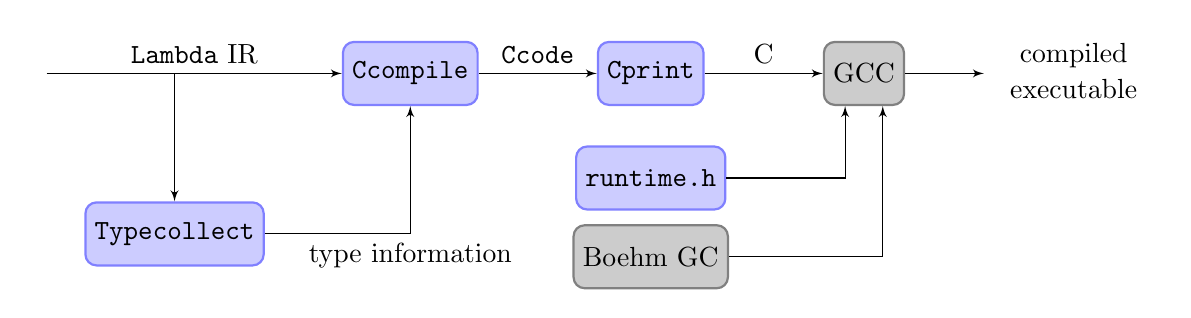
\begin{tikzpicture}[
blank/.style={node distance=1.5cm},
block/.style={rectangle, text centered, rounded corners, minimum height=0.8cm, 
node distance=1.5cm, thick, draw=blue!50, fill=blue!20},
block-emph/.style={block, draw=red!50, fill=red!20},
block-neutral/.style={block, draw=black!50, fill=black!20},
line/.style={draw, -latex'}
]
\node[blank] (start) at (0, 0) {};
\node[blank, right=1.5cm of start] (dummy) {};
\node[block, below=1.5cm of dummy] (typecollect) {\texttt{Typecollect}};
\node[block, right=2cm of dummy] (ccompile) {\texttt{Ccompile}};
\node[block, right=of ccompile] (cprint) {\texttt{Cprint}};
\node[block-neutral, right=of cprint] (gcc) {GCC};
\node[block, below=0.5cm of cprint] (runtime-h) {\texttt{runtime.h}};
\node[block-neutral, below=1.5cm of cprint] (boehm-gc) {Boehm GC};
\node[blank, right=1cm of gcc] (executable) {
    \begin{tabular}{c} compiled \\ executable \end{tabular}
};

\path [line] (start) -- (ccompile) node [midway, above] {\texttt{Lambda} IR};
\path [line] (dummy.center) -- (typecollect);
\path [line] (typecollect) -| (ccompile) node [midway, below] {type information};
\path [line] (ccompile) -- (cprint) node [midway, above] {\texttt{Ccode}};
\path [line] (cprint) -- (gcc) node [midway, above] {C};
\path [line] (runtime-h) -| (gcc.240);
\path [line] (boehm-gc) -| (gcc.300);
\path [line] (gcc) -- (executable);
\end{tikzpicture}

    \caption{A representation of the stages in producing an executable output
    from my compiler, starting from the \texttt{Lambda} IR.}
    \label{fig:compilerpipeline}
\end{figure}

\section{Obtaining types from the \texttt{Lambda} IR} \label{lambda-types}

The \texttt{Lambda} IR does not have any type information associated with it, as
within the OCaml compiler, \texttt{Lambda} was intended as the last
representation before compilation into actual machine code, so all type
information was erased from the underlying data.

While not having types isn't such a big problem for the compilation into C, one
of the goals of the project was to have the resulting code be ``observable'',
which means where possible variables should be of a meaningful type in order to
be displayed correctly in GDB.

\subsection{\texttt{Lambda} Events} \label{levents}

The OCaml compiler inserts \texttt{Lambda} events into the \texttt{Lambda} IR
when the debug flag is set. A \texttt{Lambda} event is simply a wrapper around
another \texttt{Lambda} expression that carries some extra information, which
includes the potential type of an expression and the current location in the
source code.

Within the OCaml compiler, the purpose of a \texttt{Lambda} event is to mark
where an interesting expression may be, so that the debugger may stop execution
and inspect the state of the program just before the evaluation of the
expression, or just after. This gives \texttt{Lambda} events two main useful
properties, which are:

\begin{itemize}

\item \texttt{Lambda} events provide information about the current source code
    location of the expressions being currently compiled, which will be useful
    in for specifying source location (see \S\ref{line-directive});

\item \texttt{Lambda} events provide type information about types of certain
    expressions.

\end{itemize}

Unfortunately, the compiler does not insert events that give types for every
expression, nor is there a one-to-one correspondence between \texttt{Lambda}
expressions and source-code expressions, since the \texttt{Lambda} IR may
simplify certain expressions or insert new ones. However, every source-code
variable was associated with at least one \texttt{Lambda} event describing its
type. Therefore, determining types of variables used the \texttt{Lambda} events,
and types of compound expressions were determined with very basic type-
inference.

\subsection{The \texttt{Typecollect} module}

The \texttt{Typecollect} module therefore has a function \texttt{scrape} which
does the following:

\begin{enumerate}

    \item Initialise a hash table of variable identifiers to types
    (this is safe as the \texttt{Lambda} IR already assigns a different 
    identifier to every variable)

    \item Walk recursively down the \texttt{Lambda} tree:

    {\setlength{\itemindent}{25pt} \item Upon encountering a \texttt{Lambda} 
    event surrounding a variable:}

    {\setlength{\itemindent}{50pt} \item Set the variable and its type in the 
    hash table}

    \item Return the now-filled hash table.

\end{enumerate}

This preliminary pass over the \texttt{Lambda} IR passes the infered types to
the \texttt{Ccompile} module.

\section{Representation of C} \label{representation-c}

Before compilation can start, an appropriate representation of C must be chosen 
as the compilation target for the compiler.

\subsection{Expressions to statements} \label{expr-stmt}

OCaml is what is known as an expression-oriented programming language, where
every syntactical construct is actually an expression of some kind. This is in
contrast to C, which is statement-oriented. Contrast for example the following
(slightly contrived) piece of code in OCaml and C:

\begin{lstlisting}[language=Caml]
let sq_max_plus_one x y =
    (let m = if x > y then x else y in m * m) + 1
\end{lstlisting}

\begin{lstlisting}[language=C]
int sq_max_plus_one(int x, int y) {
    int m;
    if (x > y) {
        m = x;
    } else {
        m = y;
    }
    return m * m + 1;
}
\end{lstlisting}

To solve this problem, my compiler assigns every sub-expression in the program
to a separate variable. This means that if an expression consists of just a
variable, use the variable name directly; otherwise, create and assign the
result of each sub-expression to a new temporary variable.

By setting up a variable for each sub-expression, this creates an equivalence
between variables and sub-expressions. The compilation of any expression
therefore generates some sequence of statements, by the end of which the value
of the expression is assigned to a variable. The compilation function therefore
adds the statements to the current context, and returns the variable. 

\subsection{The \texttt{Ccode} module}

The \texttt{Ccode} module is a module of the compiler that simply stores the
type declarations for the internal representation of C. More details is given in
the appendix at \S\ref{ccode}.

\subsection{The \texttt{Cprint} module}

The \texttt{Cprint} module is another module that's fairly straightforward --
it contains functions for printing types from \texttt{Ccode} to an output
stream, most likely a file. Its functions simply recursively traverse down the
\texttt{Ccode} representation and prints out the corresponding C as it goes
along.

\subsection{\texttt{\#}\texttt{line} directives} \label{line-directive}

A key observability feature is for the debugger to associate the currently
executing machine code with the relevant line from the source.

C compilers support controlling the line and source file of your code with use
of the \texttt{\#}\texttt{line} directive. This means the compiler can put all
statements associated with one line of source on the same line\footnote{The line
    number changes whenever there is a new line, even after being specified with
\texttt{\#}\texttt{line}.}, interspersed with a \verb|#line| directive whenever
the source code line actually changes.

To actually obtain information about which line we're on, we again use
\texttt{Lambda} events (\S\ref{levents}), as they carry information about the
current file and line. Since they also represent places where the OCaml bytecode
debugger \texttt{ocamldebug} may pause execution, this gives us a pleasing way
to treat them: \texttt{Lambda} events simply compile directly into \verb|#line|
directives.

\section{Compiler basics} \label{compiler-basics}

Structures from Subset 1 were implemented first, which included basic
structures, some of which are included below. In the interest of brevity other
more trivial structures are described in the appendix at
\S\ref{basic-constructs}.

\subsection{\texttt{let} bindings}

When compiling let bindings, special attention needs to be paid to the variable
scoping (see \S\ref{variable-scoping}). In OCaml, a \texttt{let} binding has the
structure:

\begin{center}
    \texttt{let \emph{x} = \emph{expr} in \emph{body}}
\end{center}

Note that \texttt{\emph{x}} is not a free variable of \texttt{\emph{expr}} 
but is one in \texttt{\emph{body}}, and also that the value of the overall 
expression is the evaluated value of \texttt{\emph{body}}. Thus, a block is 
required to emulate the scoping correctly.

We therefore define the compilation of \texttt{let} bindings like thus, using
the notation defined in \S\ref{meta-notation}:

\begin{lstlisting}
comp<let $\emph{x}$ = $\emph{expr}$ in $\emph{body}$> :=

declare result;

comp<$\emph{expr}$>;
declare temp = var<$\emph{temp}$>;
{
    declare x;
    x = temp;
    
    comp<$\emph{body}$>;
    result = var<$\emph{body}$>;
}
\end{lstlisting}

\texttt{\emph{expr}} must be evaluated outside of the inner scope, where
\texttt{\emph{x}} is visible, and \texttt{\emph{body}} must be evaluated inside
the inner scope. We declare and assign the value of \texttt{\emph{x}} only
inside the inner scope. In addition, the actual value of \texttt{\emph{expr}}
must then be available outside the inner scope, so we propagate it outwards by
declaring a variable \texttt{result} in the outer scope and performing its
actual assignment in the inner scope.

OCaml also allows \texttt{let} bindings to be a shorthand for function
declaration; function compilation will be discussed in \S\ref{functions}.

\subsection{Recursive bindings with \texttt{let rec}}

Normally in a let binding, the variable being bound is not in scope for the
expression being bound. This however makes it difficult to define recursive
functions, so OCaml supplies the \texttt{let rec} binding which is useful for
creating recursive functions, or sets of mutually recursive functions. For
example, consider the following functions:

\begin{lstlisting}[language=Caml]
let rec add x y =
    if x = 0 then y else add (x - 1) (y + 1)

let rec even n =
    if n = 0 then true else odd (n - 1)
and odd n =
    if n = 0 then false else even (n - 1)
\end{lstlisting}

However OCaml allows \texttt{let rec} bindings to be used for creating a
restricted class of non-functional recursive values. The typical example given
is:

\begin{center}
    \texttt{let rec x = 1::y and y = 1::x in \emph{expr}}
\end{center}

This binds \texttt{x} to the infinite list \texttt{1::2::1::2::...}, which is
accomplished by making the list cyclical. Unsurprisingly, this is very rarely
used feature within OCaml, but in the interest of fully supporting all features
within our OCaml subset we would also like to compile expressions like this
correctly.

Informally, the class of values that are allowed to be used as the right-hand
side of a \texttt{let rec} binding are those where the recursively bound names
occur only within a function, or a data constructor. This means that to preserve
the semantics in C, the compiler therefore compiles \texttt{let rec} in two
phases:

\begin{itemize} 
    
\item Variables are declared. If the associated expression has no free variables
    that are bound as part of the same \texttt{let rec}, evaluation can happen
    immediately; otherwise, its size is determined and then space for them is
    allocated with \texttt{malloc}, issuing them addresses in the process.        

\item Once all addresses are known, evaluation proceeds using the obtained
    addresses in place of variables which reference a value bound in the
    \texttt{let rec}.

\end{itemize}

\section{OCaml value representation} \label{value-repr}

This section largely details work undertaken to implement Subset 2, which deals 
with data representation and the language structures surrounding them.

\subsection{Representation requirements}

Before discussing the strategy for representing OCaml values, it is useful to
discuss the problems that the value representation needs to solve.

\subsubsection{Polymorphic types}

Polymorphic code does not know the precise type of values it is manipulating, so
cannot deal with variable size data as they may not copy polymorphic values
correctly.

\subsubsection{OCaml blocks}

More complex types such as tuples and records are represented by a construct
known as an OCaml block, which is a variable length array of values with a
header containing its length and an integer tag value.

The \texttt{Lambda} IR in fact normalises all data structures into blocks, 
including references (they're a mutable singleton block), arrays, modules etc. 
which is rather convenient as we can implement all of these data types for free 
by implementing blocks.

\subsubsection{Algebraic Data Types}

A major feature in OCaml is the ADT, which combines elements of both enums and
record types. As an example, consider the following type declaration:

\begin{lstlisting}[language=Caml]
type color =
  | Red
  | Green
  | Blue
  | Gray of int
  | RGB of int * int * int
\end{lstlisting}

The data constructors (\texttt{Red}, \texttt{Green}, \texttt{Blue},
\texttt{Gray}, and \texttt{RGB}) within an ADT declaration are referred to as
variants, and the type is a union of all of these types together. In the
\texttt{Lambda} IR, data constructors that do not have any parameters are
represented as integers starting from 0 (so \texttt{Red} is 0, \texttt{Green} is
1, and \texttt{Blue} is 2), and data constructors that do are represented using
OCaml blocks, with tag values starting from 0 (so \texttt{Gray} is an OCaml
block of size 1 with tag 0, and \texttt{RGB} is an OCaml block of size 3 with
tag 1). This is the significance of the tag values -- they differentiate
between different variants in ADTs.

\begin{figure}
    \centering
    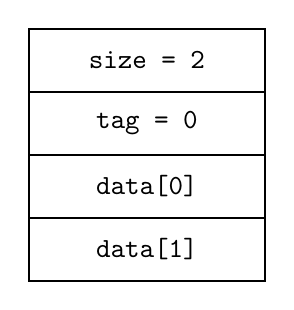
\begin{tikzpicture}[
blank/.style={node distance=0.8cm, font=\ttfamily},
block/.style={rectangle, text centered, thick, draw=black, font=\ttfamily,
    minimum width=3cm, minimum height=0.8cm, node distance=0.8cm},
block-header/.style={block, node distance=5cm},
block-body/.style={block},
line/.style={draw, thick, *-latex', shorten <=-1.2mm}
]

\node [block-header] (size) {size = 2};
\node [block-body, below of=size] (tag) {tag = 0};
\node [block-body, below of=tag] (data-0) {data[0]};
\node [block-body, below of=data-0] (data-1) {data[1]};
\end{tikzpicture}
    \caption{Example OCaml block containing two values with tag 0.}
    \label{fig:block-header}
\end{figure}

\subsection{Representation strategy}

As a consequence of the fact that we want the resulting C code to be observable,
whenever there is an exact primitive type the C code should attempt to use the
equivalent type in C as much as possible.

Representation for non-primitive types however is more complex. Integer types
and OCaml blocks must be unified in representation, because variants that don't
have any parameters and variants that do can be of the same type.

\subsubsection{Tagged pointers}

OCaml blocks must be allocated on the heap since they are of variable size, and
so have to be referenced using a pointer. This means that we need a type than
can either be a pointer or an integer, which is what tagged pointers provide.

Tagged pointers are just a union type between pointers and integers. On most
architectures, pointers are word-aligned, meaning that the lower bits of a
pointer are always 0. The tagged pointer approach employed in this compiler is
to use the least significant bit of an 8-byte word as the tag bit to
differentiate between pointers and integers, and the remaining 63 bits to store
the integer or pointer.

There is a choice as to which way round the tag bit should be -- should 0 
represent integers or pointers? I chose to use 0 for pointers, and 1 for 
integers, which means that the ``boxed'' version of a pointer is identical to 
the pointer in memory. This has the effect that dereferencing pointers is cheap
and we can use a conservative GC with no modification -- see \S\ref{gc}.

\subsubsection{Polymorphic values}

We can use the tagged pointer representation to represent polymorphic values as
well, by boxing all non-integer values into a block. To disambiguate these
blocks from other normal blocks so that at runtime, the debugger is able to see
what type they really are, we assign a special tag to them which for example
marks the block as containing only \texttt{float}s or \texttt{string}s.

\begin{figure}
    \centering
    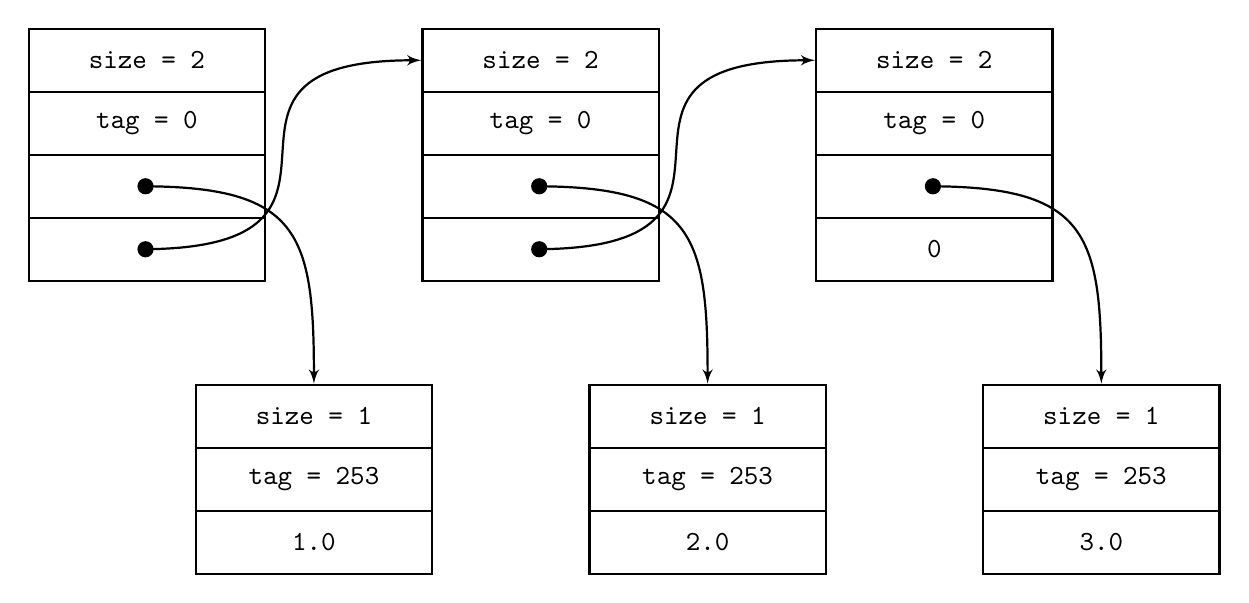
\begin{tikzpicture}[
blank/.style={node distance=0.8cm, font=\ttfamily},
block/.style={rectangle, text centered, thick, draw=black, font=\ttfamily,
    minimum width=3cm, minimum height=0.8cm, node distance=0.8cm},
block-header/.style={block, node distance=5cm},
block-body/.style={block},
line/.style={draw, thick, *-latex', shorten <=-1.2mm}
]

\node [block-header] (a-size) {size = 2};
\node [block-body, below of=a-size] (a-tag) {tag = 0};
\node [block-body, below of=a-tag] (a-data-0) {};
\node [block-body, below of=a-data-0] (a-data-1) {};

\node [block-header, right of=a-size] (b-size) {size = 2};
\node [block-body, below of=b-size] (b-tag) {tag = 0};
\node [block-body, below of=b-tag] (b-data-0) {};
\node [block-body, below of=b-data-0] (b-data-1) {};

\node [block-header, right of=b-size] (c-size) {size = 2};
\node [block-body, below of=c-size] (c-tag) {tag = 0};
\node [block-body, below of=c-tag] (c-data-0) {};
\node [block-body, below of=c-data-0] (c-data-1) {0};

\node [block-header, below right of=a-data-1, node distance=3cm] (d-size) {size 
= 1};
\node [block-body, below of=d-size] (d-tag) {tag = 253};
\node [block-body, below of=d-tag] (d-data-0) {1.0};

\node [block-header, below right of=b-data-1, node distance=3cm] (e-size) {size 
= 1};
\node [block-body, below of=e-size] (e-tag) {tag = 253};
\node [block-body, below of=e-tag] (e-data-0) {2.0};

\node [block-header, below right of=c-data-1, node distance=3cm] (f-size) {size 
= 1};
\node [block-body, below of=f-size] (f-tag) {tag = 253};
\node [block-body, below of=f-tag] (f-data-0) {3.0};

\path [line] (a-data-0.center) to [out=0, in=90, looseness=1.5] (d-size);
\path [line] (a-data-1.center) to [out=0, in=180, looseness=2] (b-size);

\path [line] (b-data-0.center) to [out=0, in=90, looseness=1.5] (e-size);
\path [line] (b-data-1.center) to [out=0, in=180, looseness=2] (c-size);

\path [line] (c-data-0.center) to [out=0, in=90, looseness=1.5] (f-size);

\end{tikzpicture}
    \caption{Example box-and-pointer diagram for the list \texttt{[1.0; 2.0;
        3.0]}. Floating point numbers must be boxed to be stored in a block, so
        a special block is created for each one with the special tag 253.}
    \label{fig:block-example}
\end{figure}

\subsection{Representation in C} \label{c-repr}

By taking advantage of flexible array members, it is easy to implement an OCaml 
block in C.

\begin{lstlisting}[language=C]
typedef struct _block {
    uintptr_t size : 56;
    uintptr_t tag : 8;
    any_type data[];
} block;
\end{lstlisting}

Recall that a block needs to store its size, an integer tag, and any number of
other OCaml values. Since OCaml tags only range between 0-255\footnote{In fact,
    the native OCaml runtime restricts the number of possible variants to 246,
    using the tags 0-245 for variants. It uses the last 10 possible tags for
special tags.}, and 45 bits are sufficient for storing the size of a block in
words, we can reduce the amount of space used for the header using C bit-fields.
This means the header only needs to be one word long.

We can now implement actual OCaml values as a union type:

\begin{lstlisting}[language=C]
typedef union _value_type {
    intptr_t i;
    block* block;
} value_type;

#define BOX_INT(v) ((value_type){.i = (intptr_t)(v) << 1 | 1})
#define UNBOX_INT(v) ((v).i >> 1)

#define BOX_BLOCK ((value_type){.block = (v)})
#define UNBOX_BLOCK ((v).block)

#define IS_INT(v) ((v).i & 1)
\end{lstlisting}

\verb|BOX_INT| and \verb|UNBOX_INT| demonstrate how to box integers into a 
\verb|value_type|, and likewise for block pointers. We also have a special 
macro \verb|IS_INT|, which checks if a \verb|value_type| is holding an integer 
or a pointer -- it simply checks the last bit, returning 1 if the last bit is 
also a 1.

\subsubsection{Type-punning with \texttt{any\char`_type}}

While \texttt{block}s normally hold an array of other \verb|value_type|s, we
would like to have special blocks that represent the result of boxing certain
other primitive types, such as \texttt{float}s and \texttt{strings}. To do this,
we declare a union type \verb|any_type|\footnote{For clarity, we ignore the
problems associated with recursive type definitions in C, assuming the correct
forward declarations.}:

\begin{lstlisting}[language=C]
typedef union {
    double fl;
    char* str;
    value_type value;
} any_type;
\end{lstlisting}

We refer the act of casting one of these types to an \verb|any_type| as
``packing'', or ``unpacking'' for the opposite direction. Note that since this
is a union type, the ``pack'' operations don't represent any actual operations
in machine code.

\texttt{block} therefore declares a \verb|any_type| array to support both
storing \verb|value_type|s as well as special blocks that store \verb|double|s
and \verb|char*|s.

\subsection{Conversion between C types} \label{casting}

Despite the \texttt{Lambda} IR having already gone through type inferencing,
there are still a few cases in which ``casting'' is necessary. This is because,
for example, the C types for polymorphic types and monomorphic types in OCaml
are different, so a C cast is necessary when passing a value of a known type to
a polymorphic function.

In general, there are several cases where we need to perform a conversion
operation in C. These cases are: 

\begin{itemize}

\item A conversion from an integer to an OCaml value is required, because the
    \texttt{Lambda} IR uses integers for representing certain non-integer OCaml
    values.

\item A conversion from any other type to an OCaml value, because a variable is
    being passed into a polymorphic function, or being placed into a block.

\item An actual conversion between types, such as from integers to floating
    point numbers.

\end{itemize}

The cases all involve a mismatch between the C types of two expressions, so are
handled using a function that does the following:

\begin{enumerate}

\item If the source and target types are the same, do nothing.

\item If either type is \verb|any_type|, pack or unpack the value as
    appropriate. 

\item If either type is \verb|value_type|, box or unbox the value as
    appropriate.

\item Otherwise, perform a C cast between source type and target type.

\end{enumerate}

\subsection{Pattern matching}

OCaml employs pattern matching in many constructs of the language, particularly
in its \texttt{match} expressions. Fortunately, the \texttt{Lambda} IR usually
compiles these down to an equivalent set of \texttt{if} expressions and
\texttt{let} bindings. In the case of variants however, pattern matching
typically compiles down into a \texttt{Lswitch} expression.

\subsubsection{\texttt{Lswitch} expressions}

\texttt{Lswitch} expressions correspond to match statements on a variant 
expression. For an example, consider the type and match expression:

\begin{lstlisting}[language=Caml]
type color =
  | Red
  | Green
  | Blue
  | Gray of int
  | RGB of int * int * int

match c with
  | Red -> 0
  | Green -> 1
  | Blue -> 2
  | Gray x -> 3
  | RGB (r, g, b) -> 4
\end{lstlisting}

This match statement is compiled into the following \texttt{Lambda} expression:

\begin{lstlisting}
(switch* c/xxxx
  case int 0: 0
  case int 1: 1
  case int 2: 2
  case tag 0: 3
  case tag 1: 4)
\end{lstlisting}

There's one important difference between this and a C switch statement: each of
the cases predicate on both whether the value is an integer or a block in
addition to its value or tag.

One \texttt{Lswitch} statement therefore compiles into two switch statements in
C, one for the integers and one for the tags, which are the two branches of an
if statement that checks if the value being switched on is an integer or a value
using the tagged pointer check.

\section{Function compilation and closure conversion} \label{functions}

Functions and closures are the final major feature required to compile the
target subset of OCaml into C. The following sections will discuss the
motivations for a closure representation and the implementation of such a
representation, which is the majority of work undertaken in the implementation
of Subset 3.

\subsection{Local functions}

All functions in C are required to be defined at top-level, which means that 
nested function declarations are not possible. This is in contrast to OCaml, 
where function definitions are simply expressions like any other, and thus can 
be defined locally and passed as values. In order to emulate this behaviour in 
C, whenever we come across a function definition we lift the function 
definition to the toplevel scope, compile the function there, and then return 
its function pointer when we come back.\footnote{This clearly does not deal 
with lexical closures, so we actually return a pointer to a closure object 
instead of a function pointer, but the idea is the same.}

We can write the compilation of a local function like thus, using the notation
from \S\ref{meta-notation}:

\begin{lstlisting}
comp<fun $\emph{args...}$ -> $\emph{body}$> :=

/* in top-level */
$\emph{return\char`_type}$ local_function($\emph{args...}$) {
    comp<$\emph{body}$>;
    return var<$\emph{body}$>;
}

/* in current context */
declare result = &local_function;
\end{lstlisting}

\subsection{Function Types in C} \label{function-typing}

In OCaml, one way of viewing functions is always as functions of one argument,
which can return other functions. As an example, the function type \texttt{int
-> float -> int} represents a function that takes an integer and returns a
\texttt{float -> int}, which is a function that takes a floating point number
and returns an integer.

While this is a correct high-level view of functions, this is not suitable for a
low-level implementation at all, since it is much more efficient for functions
to actually accept multiple arguments instead of taking one argument at a time.

In C by contrast, a function declaration consists of a return type, and a list 
of input arguments. We therefore need a consistent conversion between OCaml 
function types and C function types, so we pick the most obvious one -- all the 
types in the OCaml function type are the arguments to the C function, and the 
final type is the return type of the C function.

For example, a function of type \texttt{int -> float -> str} is compiled to
\texttt{char* (*)(int, double)} in C.

\subsection{Closure representation}

Closures are, implementation-wise, a structure that stores both a function 
pointer and an environment, containing values required for the execution of the 
function.

Our closure representation essentially requires storing a function pointer and 
some list of values, so taking advantage of flexible array members again we 
arrive at the following definition:

\begin{lstlisting}[language=C]
typedef struct _closure_type {
    void* (*f)();
    struct _closure_type* next;
    any_type$\footnotemark$ args[];
}
\end{lstlisting}

\footnotetext{Note that we are reusing \texttt{any\char`_type}, which means we
need to extend its definition and the casting rules to accept more types, such
as integers, function pointers, and closure types.}

As you can see, this definition contains a function pointer, and a
variably-sized array of arguments, which we reused \verb|any_type| from
\S\ref{c-repr} to implement. Closures also have a \texttt{next} field which
points to another \verb|closure_type|, allowing them to act like a linked list.
The motivation of this is discussed in partial application compilation, in
\S\ref{partial-app}.

\subsubsection{Using closure objects}

In order to make the closure object useful, we modify all functions to instead
take an extra parameter, \texttt{closure\char`_type* closure\char`_obj}, which
stores the pointer to the current closure object. From there, the function is
able to access closure values by indexing \verb|closure_obj->args|.

Calling a closure can be done by invoking the function pointer with the 
required arguments, passing in the closure pointer as the last argument.

\begin{lstlisting}[language=C]
cl->f($\emph{args...}$, cl);
\end{lstlisting}

\subsubsection{Promoting ordinary functions to closures}

This necessitates some sort of promotion process where functions that do not
require environment capture are promoted to closures. This is done by creating
another function which takes all the same arguments as the original function
plus the closure object. This function just passes the arguments along to the
original function.

\begin{lstlisting}[language=C]
$\emph{return\char`_type}$ promoted_closure($\emph{args...}$, closure_type* closure_obj) {
    return f($\emph{args...}$);
}

closure_type* cl = MALLOC(sizeof(closure_type));
cl->f = (void*(*)())&promoted_closure;
cl->next = NULL;
\end{lstlisting}

\subsubsection{Unification of closures and functions}

For ease of representation, it was decided to unify functions and closures in C
as well. This means that all functions are promoted to closures, and all
function applications in OCaml are compiled into closure calls in C, simplifying
the implementation at the cost of possible performance losses.

\subsection{Partial application compilation} \label{partial-app}

Partial application is one of the major use-cases for closures, and is modelled
in my compiler using a closure object. Whenever there is a partial application,
a function is created instead that takes the remaining parameters, and a closure
object is created to store the partially-applied arguments. The newly created
function simply obtains the previously partially applied arguments from the
closure object and passes them along with its own arguments to reconstruct the
original function call.

As an example, observe the following C-style pseudocode, where a closure
\texttt{cl\char`_f} (which requires three integer arguments and returns an
integer) is partially applied with two integers, \texttt{a} and \texttt{b}, and
another closure \texttt{cl\char`_g} is returned\footnote{Cast operators have
been omitted for simplicity.}.

\begin{lstlisting}[language=C]
int g(int c, closure_type* closure_obj) {
    int arg_0 = closure_obj->data[0];
    int arg_1 = closure_obj->data[1];
    
    closure_type* cl = closure_obj->next;
    cl->f(arg_0, arg_1, c, cl);
}

closure_type* cl_g = MALLOC(sizeof(closure_type) + sizeof(any_type)*2);
cl_g->f = &g;
cl_g->next = cl_f;
cl_g->data[0] = a;
cl_g->data[1] = b;
\end{lstlisting}

\begin{figure}
    \centering
    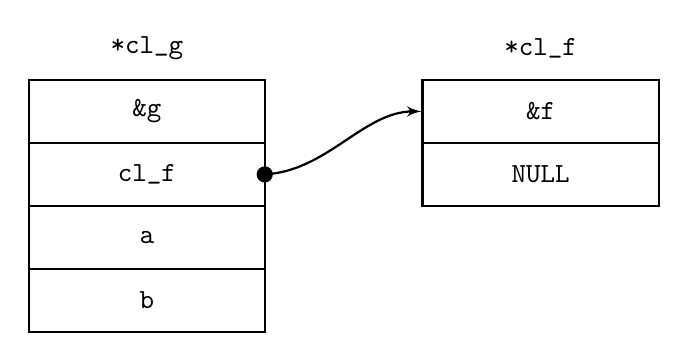
\begin{tikzpicture}[
blank/.style={node distance=0.8cm, font=\ttfamily},
block/.style={rectangle, text centered, thick, draw=black, font=\ttfamily,
minimum width=3cm, minimum height=0.8cm, node distance=0.8cm},
block-header/.style={block, node distance=5cm},
block-body/.style={block},
line/.style={draw, thick, *-latex', shorten <=-1.2mm}
]

\node [block-header] (g) {\&g};
\node [blank, above of=g] (cl-g) {\verb|*cl_g|};
\node [block-body, below of=g] (g-next) {\verb|cl_f|};
\node [block-body, below of=g-next] (a) {a};
\node [block-body, below of=a] (b) {b};

\node [block-header, right of=g] (f) {\&f};
\node [blank, above of=f] (cl-f) {\verb|*cl_f|};
\node [block-body, below of=f] (f-next) {NULL};

\path [line] (g-next) edge[out=0, in=180, looseness=.9] (f);

\end{tikzpicture}
    \caption{Example result of a partial application of a function \texttt{f(a, 
    b, c)} with the arguments \texttt{(a, b)}. The arguments \texttt{a} and 
    \texttt{b} are pushed onto a new closure object, which contains a function 
    pointer to \texttt{g} and a pointer to the previous closure object. When 
    \texttt{cl\char`_g} is called with an argument \texttt{c}, \texttt{g} will 
    obtain \texttt{a} and \texttt{b} from the closure object and pass them 
    together with \texttt{c} to \texttt{f}.}
    \label{fig:partial-app}
\end{figure}

\subsubsection{Chaining partial applications}

An important requirement is that a partially applied closure needs to act the
same as an unapplied closure, as in we must be able to partially apply it again.
This requirement is the justification for why closures are implemented as 
a linked list -- each closure needs to know the function pointer of the next 
function they need to invoke, but that isn't always possible to determine 
statically\footnote{As an example, consider a partially applied function which 
is passed as an argument to a higher-order function, which further partially 
applies the function.}.

Thus, each closure resulting from partial application points to the closure from
which it was derived from so their function can figure out what function pointer
to invoke (see figure~\ref{fig:partial-app}).

\begin{figure}
    \centering
    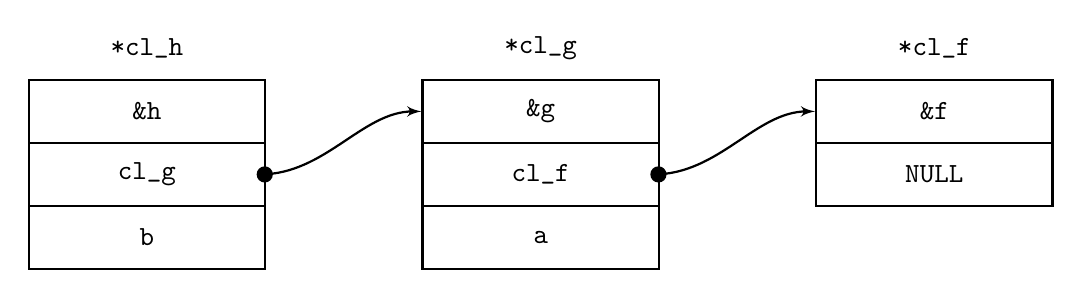
\begin{tikzpicture}[
blank/.style={node distance=0.8cm, font=\ttfamily},
block/.style={rectangle, text centered, thick, draw=black, font=\ttfamily,
minimum width=3cm, minimum height=0.8cm, node distance=0.8cm},
block-header/.style={block, node distance=5cm},
block-body/.style={block},
line/.style={draw, thick, *-latex', shorten <=-1.2mm}
]

\node [block-header] (h) {\&h};
\node [blank, above of=h] (cl-h) {\verb|*cl_h|};
\node [block-body, below of=h] (h-next) {\verb|cl_g|};
\node [block-body, below of=h-next] (b) {b};

\node [block-header, right of=h] (g) {\&g};
\node [blank, above of=g] (cl-g) {\verb|*cl_g|};
\node [block-body, below of=g] (g-next) {\verb|cl_f|};
\node [block-body, below of=g-next] (a) {a};

\node [block-header, right of=g] (f) {\&f};
\node [blank, above of=f] (cl-f) {\verb|*cl_f|};
\node [block-body, below of=f] (f-next) {NULL};

\path [line] (h-next) edge[out=0, in=180, looseness=.9] (g);
\path [line] (g-next) edge[out=0, in=180, looseness=.9] (f);

\end{tikzpicture}
    \caption{Example of a chained double application. In this case, the 
    function \texttt{f(a, b, c)} has been applied with \texttt{a} and 
    \texttt{b} separately, creating two closure objects, \texttt{cl\char`_g} in 
    the first application, and \texttt{cl\char`_h} in the second. Here, 
    \texttt{h} translates a call \texttt{h(c)} into \texttt{g(b, c)}, which in 
    turn translates that call into \texttt{f(a, b, c)}.}
    \label{fig:double-partial-app}
\end{figure}

\subsection{Lexical closure compilation}

Lexical closures are another common use of closures, and occur when a function
refers to values in an enclosing scope. This presents a problem in C, as it does
not allow nesting functions.

Because our closure representation allows storing arbitrary data already, this
is simple to implement using closure objects. When compiling any local function,
first check if the function contains any free variables. If it does, take the
value of all the free variables at that point and push them onto the closure
object, and when compiling the function body, before compiling re-assign all
lexically bound variables to values from the closure object.

As an example, consider the compilation of the following OCaml 
code:\footnote{In an actual compilation, this will get eta-expanded to make the 
function types consistent (see \S\ref{incomplete-funcs}) but we suppose 
this doesn't happen in this example for simplicity.}

\begin{lstlisting}[language=Caml]
let f x y =
    let g z = x + y + z in g
\end{lstlisting}

This is compiled into the following C-style pseudocode:

\begin{lstlisting}[language=C]
int f(int x, int y, closure_type* closure_obj) {
    closure_type* cl_g = MALLOC(sizeof(closure_type) + sizeof(any_type)*2);
    cl_g->f = &g;
    cl_g->next = NULL;
    cl_g->data[0] = x;
    cl_g->data[1] = y;
    
    return cl_g;
}

int g(int z, closure_type* closure_obj) {
    int x = closure_obj->data[0];
    int y = closure_obj->data[1];
    
    return x + y + z;
}
\end{lstlisting}

\subsection{Parametric polymorphism}

Parametric polymorphism is an important feature in OCaml, allowing programmers
to write general code without knowing the type of its arguments in advance. As
discussed in \S\ref{value-repr} we use the \verb|value_type| representation of
polymorphic values when defining polymorphic functions.

This works fine for passing simple values and polymorphic datatypes, as long as 
we remember to cast values to \verb|value_type| when passing values to 
polymorphic functions, and cast back to their actual types when receiving 
values from function calls.

However, passing other functions (closures) into polymorphic functions is more 
problematic.

\subsubsection{Erasing function types}

When passing a non-polymorphic function, e.g. \texttt{float -> float}, to
polymorphic function expecting an \texttt{'a -> 'b} requires a cast between the
two types. This is because the polymorphic function is representing \texttt{'a}
as \verb|value_type|, and so will attempt to pass data of the type
\verb|value_type| into the function, and will expect a return type also of
\verb|value_type|. Thus in order to cast \texttt{float -> float} we will need to
add a wrapper function which performs the casts.

\begin{lstlisting}[language=C]
value_type g(value_type x, closure_type* closure_obj) {
    double new_x = UNBOX_FLOAT(x);

    closure_type* cl = closure_obj->next;
    double result = cl->f(new_x, cl);
    
    value_type new_result = BOX_FLOAT(result);
    return new_result;
}

closure_type* cl_g = MALLOC(sizeof(closure_type));
cl_g->f = &g;
cl_g->next = cl_f;
\end{lstlisting}

This in fact needs to happen any time it's possible to ``lose track'' of the
actual type of a function, i.e. it's possible the function will be used in a
situation where its type has been generalised away. This includes adding
functions to an OCaml block (because the data structure may be passed to a
function polymorphic in a subtype of the data structure), or accessing functions
from an OCaml block\footnote{It's not safe to simply remove the head from the
    closure chain to undo this cast, as there's no guarantee the last
transformation applied to a closure will be the cast -- the closure may have
been partially applied or cast again to something else.}, or storing and
retrieving functions from closure data.

Thus, the casting rules from \S\ref{casting} need to be modified.

\begin{enumerate}

\item If the source type is \verb|value_type| or \verb|any_type|, when casting
    back assume all of its argument and return types are \verb|value_type|, and
    then cast it back to the expected type using the technique from the previous
    section.

\item If the target type is \verb|value_type| or \verb|any_type| and the source
    type is a function, first erase types from that function by rewriting all
    its argument and return types to \verb|value_type| using the technique from
    the previous section before proceeding with the cast.

\end{enumerate}

\subsubsection{``Upcasting'' functions}

Another case when dealing with polymorphic functions is when the expected type
of a function has fewer parameters than the actual type, e.g.  passing a
function of type \texttt{float -> float -> float} to a higher-order function
that is expecting a \texttt{'a -> 'b}. This poses a problem for the type system
for functions we decided on in \S\ref{function-typing}.

To see why, consider a polymorphic function which receives a function 
\texttt{'a -> 'b}, and needs to apply it to something of type \texttt{'a}. How 
does it know whether to treat this as a full application, where it needs to 
invoke the function as a closure, or a partial application, where it needs to 
create a new closure object?

One solution is to solve this on the caller's side. Essentially, we want to
transform a C function signature from:

\begin{lstlisting}[language=C]
value_type f(value_type x, value_type y, closure_type* closure_obj);
\end{lstlisting}

into\footnote{The \texttt{closure\char`_type*} is actually also cast into a 
\texttt{value\char`_type}, to match the type the polymorphic function is 
expecting.}:

\begin{lstlisting}[language=C]
closure_type* g(value_type x, closure_type* closure_obj);
// where the returned value points to the function
value_type h(value_type y, closure_type& closure_obj);
\end{lstlisting}

This is to ensure that from the point of view of a polymorphic function, if the 
same number of elements is applied to the function type, then it can be 
considered fully applied.

This transformation can be modelled using the current closure representation,
using a process I refer to as ``upcasting''. In this process of upcasting a
function \texttt{f}, two more functions are created, which are \texttt{g} and
\texttt{h}.

\texttt{g}'s role is to act as the resulting function that will be passed into
whatever polymorphic function. It's essentially a wrapper around a partial
application.

\begin{lstlisting}[language=C]
closure_type* g(value_type x, closure_type* closure_obj) {
    closure_type* cl = MALLOC(sizeof(closure_type) + sizeof(any_type));
    cl->f = &h;
    cl->next = closure_obj;
    cl->data[0] = x;
    
    return cl;
}
\end{lstlisting}

\texttt{h} acts as the counterpart function to a polymorphic function, which 
takes the data that \texttt{g} has set up for it and applies it to \texttt{f}.

\begin{lstlisting}[language=C]
value_type h(value_type y, closure_type* closure_obj) {
    value_type x = closure_obj->data[0];
    
    closure_type* cl = closure_obj->next;
    value_type result = cl->f(x, y, cl);
    
    return result;
}
\end{lstlisting}

The surrounding code adds \texttt{g} as a closure onto \texttt{f}'s closure.

\begin{lstlisting}[language=C]
closure_type* cl_g = MALLOC(sizeof(closure_type));
cl_g->f = &g;
cl_g->next = cl_f;
\end{lstlisting}

By tracing through the executions, it can be seen that an application by 
\texttt{x} followed by an application by \texttt{y} gives the correct function 
call \texttt{f(x, y)}.

\section{Garbage Collection} \label{gc}

We can use the Boehm GC to implement a garbage collector without needing to
write one ourselves. Because of the way we have defined the implementation of
OCaml values, all values potentially representing pointers will be unchanged in
their actual binary value. This means that we can simply ``drop-in'' the Boehm
GC by including the following in our runtime:

\begin{lstlisting}[language=C]
#include "gc.h"
#define MALLOC(v) GC_MALLOC(v)
\end{lstlisting}

\chapter{Evaluation}

The resulting compiler was evaluated in two key aspects, which are the 
resulting speed of the produced executables and the observability of the debug 
output. \S\ref{regression-tests} talks about regression tests used to test the
correctness of the compiler, \S\ref{benchmarks} presents results and analyses
about the speed of compiled executables, and \S\ref{observability} compares the
observability of compiled executables with that of the OCaml debugger.

The benchmark results are quite favourable -- despite not much effort being put
in to optimise the output of the compiler, the resulting executables frequently
perform as well as, if not better than, as the OCaml native compiler, although
for certain workloads they perform much worse. The observability results show
that basic observability features are possible, and in fact exceed the OCaml
debugger in some cases.

\section{Regression tests and feature completeness} \label{regression-tests}

To test the correctness of the compilation, 21 different regression tests were
written, testing if different features of the language were being compiled
correctly. They include simple tests which test one feature each, to more
complex tests which test multiple features combined in different variations.

With every iteration of the compiler, regression tests are run against it to 
ensure that the output of the compiler remains correct. To do this, a simple 
regression test script was written which compiles the same OCaml program 
against the OCaml native compiler and my compiler, and asserts that the output 
of both executables match.

\section{Benchmarks} \label{benchmarks}

One natural way of evaluating the compiler is to compare the execution times of
its output against the output of the OCaml compilers. Therefore, for the
evaluation we should compile the \emph{same OCaml program} against both my
compiler and the OCaml compiler, and then compare the execution speed outputs.

Several different configurations for comparisons can be attempted. OCaml
supplies two compiler backends, the OCaml native compiler (\texttt{ocamlopt})
and the OCaml bytecode compiler (\texttt{ocamlc}). For our purposes, we will be
mostly considering the output of the native compiler, as the bytecode
interpreter is at least one order of magnitude slower.

In addition, since my compiler produces C code we have a choice as to which
compiler to compile the C code with, and under which configurations. I chose the
most popular C compilers, \texttt{gcc} and \texttt{clang}, and compiled the code
under the four optimisation levels provided (\texttt{-O0}, \texttt{-O1},
\texttt{-O2}, and \texttt{-O3}).

To simplify the process of running the many benchmarks against the
configurations, a script \texttt{run\char`_benchmarks.py} was written, and the
results were plotted using Python and matplotlib.

\subsection{Sourcing Benchmarks}

Benchmarks programs were taken from the Computer Language Benchmarks Game
(CLBG)\footnote{\url{https://benchmarksgame-team.pages.debian.net/benchmarksgame/}},
the \texttt{operf-micro}\footnote{\url{https://github.com/OCamlPro/operf-micro}}
OCaml library, and the rest were written by me.  They were chosen to exemplify a
wide range of features within the OCaml language, particularly to exercise the
more advanced features of the subset of OCaml which I am targeting.

Benchmarks were adjusted to take between 0.5 to 2.0 seconds to run so that the
timer does not significantly affect the running time, and were run 50 times each
on an idle Linux laptop.

\begin{figure}
    \centering
    \resizebox{\textwidth}{!}{
        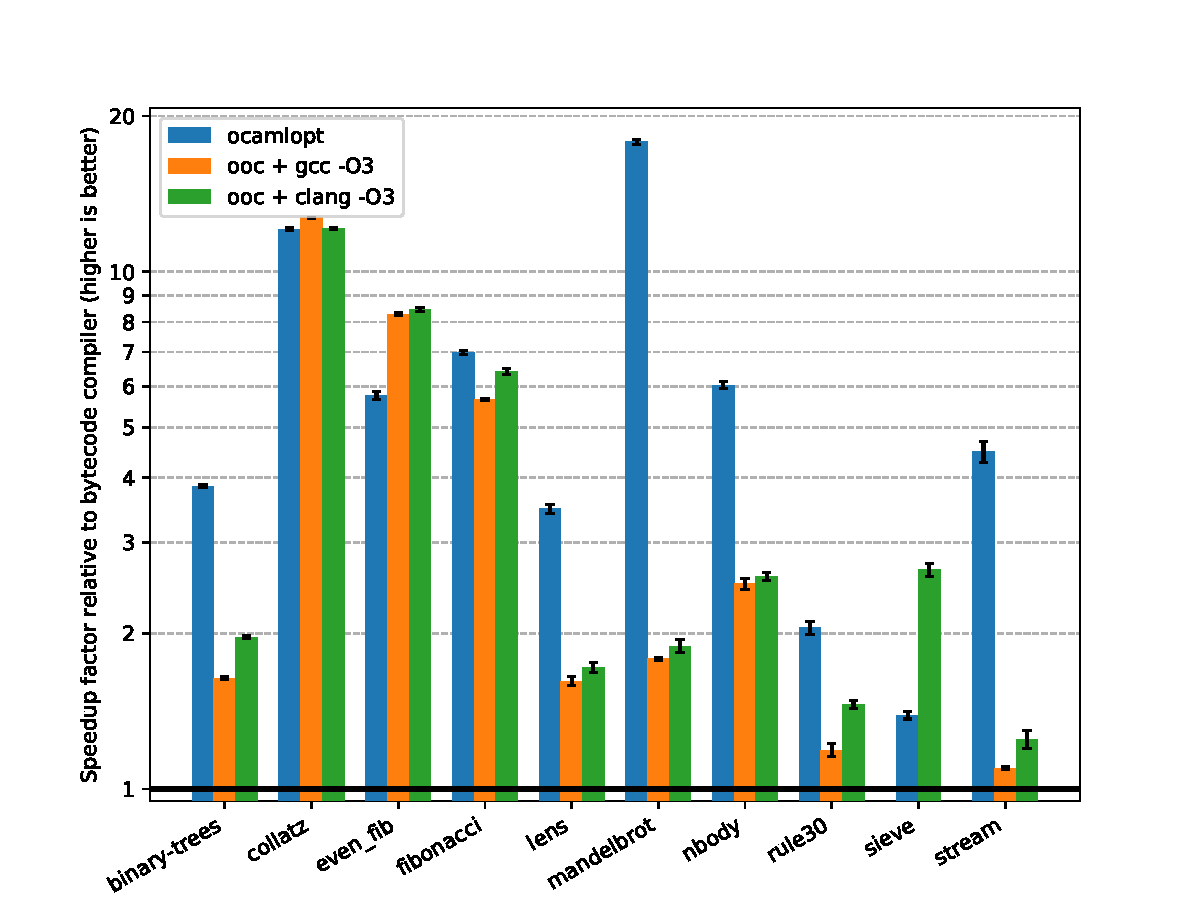
\includegraphics{figs/raw_benchmarks.pdf}
    }

    \caption{
    Comparison of speed-ups in terms of execution time, compared to the OCaml
    bytecode compiler. Higher is better. The compared executables were the
    outputs of the OCaml native compiler (\texttt{ocamlopt}), the OCaml bytecode
    compiler (\texttt{ocamlc}), my compiler (referred to as the Observable OCaml
    Compiler, or \texttt{ooc}) in combination with \texttt{gcc} and
    \texttt{clang}. The black line represents the baseline of the OCaml bytecode
    compiler, and error bars represent 1 standard deviation in the results.
    }
    
    \label{fig:raw-benchmarks}
\end{figure}

On the whole, C compilers do quite well in comparison to the OCaml native
compiler being only a small constant factor time slower in most cases and
matching and even outperforming the native compiler in select cases. Also for
all benchmarks, the C compilers outperformed the OCaml bytecode compiler, which
is surprising since no significant effort was made into optimisation of the C
output.

Notable results from the benchmark include:

\begin{itemize}

\item The drop-in Boehm garbage collector is unsurprisingly much slower than the
    OCaml GC, as it is a conservative GC and does not have any domain-specific
    knowledge. This can be best seen in the \texttt{binary-trees} benchmark.

\item The C compilers perform extremely well on benchmarks that involve few
    allocations and straightforward tail-recursive code, often beating even the
    OCaml native compiler. This is seen in the \texttt{collatz},
    \texttt{even\char`_fib}, and \texttt{sieve} benchmarks.

\item Strangely, the C compilers perform exceptionally badly in benchmarks
    involving floating point manipulations, as can be seen in
    \texttt{mandelbrot} and \texttt{nbody} benchmarks. This is investigated in
    \S\ref{float-alloc}.

\item Benchmarks which involve lots of closure creation and application are also
    slower relative to the OCaml native compiler, as can bee seen in the
    \texttt{lens} and \texttt{stream} benchmarks.

\item In the \texttt{sieve} benchmark, the executable compiled with \texttt{gcc}
    actually segfaults, the cause of which is a failure to perform a tail-call
    optimisation. This is discussed further in \S\ref{stack-overflow}.

\end{itemize}

\subsection{Investigating performance differences}

\subsubsection{Instrumentation}

The obvious next step after obtaining results for the benchmarks is to perform
an investigation into the performance differences; we would like some way of
profiling the code to see what parts of the code take longer to run.

Fortunately, a key consequence of the compiler being from OCaml to C is that
standard C tools will work on the resulting code. This includes Gprof, a
profiler which can be enabled in \texttt{gcc} with the \texttt{-pg} flag. Gprof
can provide information as to how much time is spent in each function via the
flat profile, as well as information about how the call graph, or which
functions called what other functions and how many times.

OCaml also supports using Gprof to profile its native code output simply by
adding the \texttt{-p} flag to \texttt{ocamlopt}, giving us a convenient way to
compare the execution of the C executable and the OCaml native executable. We
can therefore use this profiler to investigate performance differences between
the OCaml native compiler and the C compiler.

\subsubsection{Floating point and polymorphic structures} \label{float-alloc}

For example, one discrepancy which we may wish to investigate is the 
\texttt{mandelbrot} benchmark, which C compilers perform much worse on despite 
having been written in imperative-style code.

\begin{figure}
    \centering
    \texttt{ocamlopt}
\begin{lstlisting}[basicstyle=\ttfamily\footnotesize,
basewidth={.5em,.3em}, frame=single]
  %   cumulative   self              self     total           
 time   seconds   seconds    calls  ms/call  ms/call  name    
100.00      0.93     0.93        1   930.03   930.03  $\cbox{green!25}{camlTest\char`_\char`_entry}$
  0.00      0.93     0.00  1125001     0.00     0.00  $\cbox{green!25}{caml\char`_ml\char`_output\char`_char}$
  0.00      0.93     0.00  1125000     0.00     0.00  $\cbox{green!25}{camlTest\char`_\char`_print\char`_byte\char`_1232}$
  0.00      0.93     0.00     1489     0.00     0.00  caml_page_table_modify
  0.00      0.93     0.00       28     0.00     0.00  caml_stat_alloc
...
\end{lstlisting}
\texttt{ooc + gcc -O3}
\begin{lstlisting}[basicstyle=\ttfamily\footnotesize,
basewidth={.5em,.3em}, frame=single]
  %   cumulative   self              self     total           
 time   seconds   seconds    calls  ms/call  ms/call  name    
 44.37      7.00     7.00                             $\cbox{green!25}{main}$
 10.65      8.68     1.68 676990954     0.00     0.00  $\cbox{red!25}{BOX\char`_GEN}$
  8.71     10.06     1.38                             $\cbox{red!25}{GC\char`_malloc\char`_kind}$
  8.24     11.36     1.30                             $\cbox{blue!25}{GC\char`_build\char`_fl}$
  7.16     12.49     1.13                             $\cbox{blue!25}{GC\char`_apply\char`_to\char`_all\char`_blocks}$
  3.55     13.05     0.56                             $\cbox{blue!25}{GC\char`_mark\char`_from}$
  2.66     13.47     0.42                             $\cbox{red!25}{GC\char`_allochblk\char`_nth}$
  2.28     13.83     0.36                             $\cbox{blue!25}{GC\char`_clear\char`_stack\char`_inner}$
  1.77     14.11     0.28                             frame_dummy
  1.71     14.38     0.27                             $\cbox{blue!25}{GC\char`_reclaim\char`_clear}$
  1.05     14.54     0.17                             $\cbox{red!25}{GC\char`_malloc}$
  0.76     14.66     0.12                             $\cbox{blue!25}{GC\char`_find\char`_header}$
  0.63     14.76     0.10                             $\cbox{blue!25}{GC\char`_clear\char`_hdr\char`_marks}$
  0.63     14.86     0.10                             $\cbox{blue!25}{GC\char`_finish\char`_collection}$
  0.48     14.94     0.08                             $\cbox{red!25}{GC\char`_generic\char`_malloc\char`_inner}$
...
\end{lstlisting}

    \caption{Truncated Gprof outputs for the OCaml native executable and the C
        executable for the \texttt{mandelbrot} benchmark, which has been
        highlighted with the roles of each function.  Functions highlighted
        green are logical functions for the execution of the program, functions
        highlighted red are to do with allocating blocks on the heap, and
        functions highlighted blue are functions used by the garbage collector.
        Note that compiling with profiling information inserts extra
        instructions and function calls for instrumentation purposes so the
        times shown are not indicative of how fast the benchmarks execute
        otherwise.}
    \label{fig:mandelbrot-gprof}
\end{figure}

I collected profiling information using Gprof from both the native and C
executables, a truncated version of which\footnote{Since the full output from
Gprof is not as useful, the reports have been truncated so that at least the top
95\% of the execution time is represented.} can be seen in
figure~\ref{fig:mandelbrot-gprof}. As shown, the OCaml executable spends almost
100\% of its execution time in the main logic of the program (which is the
\texttt{entry} function), in comparison to the C executable, which only spends
44.37\% of the execution time in the main logic. Instead, the majority of the
time spent during execution is allocating new blocks and garbage collecting old
ones.

Upon further investigation, it was found that the \texttt{mandelbrot} benchmark
stored \texttt{float}s inside \texttt{float ref}s, and the \texttt{Lambda}
representation normalises references into singleton OCaml blocks. This means
that according to the casting rules as described in \S\ref{casting}, whenever a
\texttt{float} needs to be stored inside a \texttt{float ref} a new tagged OCaml
block is allocated on the heap and then the pointer is stored in the
\texttt{float ref}. This means that mutable floating point fields within OCaml
blocks are in fact incredibly slow, as each store necessitates creating a new
block on the heap, and needing to GC the block that was replaced.

The same is true for the \texttt{nbody} benchmark, which uses mutable float 
fields in a record to store the position, velocity, mass etc. of the different 
celestial bodies.

This unfortunately makes floating point operations very slow, and a solution is
attempted for this in \S\ref{reduced-allocs}.

\subsubsection{Tail recursion} \label{tail-recursion}

Another interesting question to ask is if the C compilers can see through the 
closure representation to perform tail-call optimisation, since it is far more 
idiomatic to write tail-recursive functions in OCaml than it is to write 
explicit iteration. It is therefore important for performance that the C 
compilers can do tail-call optimisation to avoid the extra overheads of 
function calls as well as avoiding stack overflows.

To do this, we can use the \texttt{objdump} Linux utility, which can 
``disassemble'' the executable, printing out the assembly mnemonics 
corresponding to the machine code.  Figure~\ref{fig:tail-recursion} shows the 
disassembly of the following simple tail-recursive function:

\begin{lstlisting}[language=Caml]
let rec add x y =
  if y = 0 then
    x
  else
    add (x - 1) (y + 1)
\end{lstlisting}

As can be seen, the C compiler is able to infer that the closure application is 
equivalent to a function call in tail-call position, despite not being able to 
see through the closure representation explicitly, and has therefore compiled 
the closure application into a single \texttt{jmp} instruction. This means that 
tail-recursive functions do not incur the full penalties from a function call, 
but a small amount of overhead from needing to load in an address.

\begin{figure}
    \centering
    \begin{lstlisting}[basicstyle=\ttfamily\footnotesize,
basewidth={.5em,.3em}, frame=single]
0000000000400fe0 <local_func_1215>:
  400fe0:       48 85 f6                test   rsi,rsi
  400fe3:       75 0b                   jne    400ff0 <local_func_1215+0x10>
  400fe5:       48 89 f8                mov    rax,rdi
  400fe8:       c3                      ret    
  400fe9:       0f 1f 80 00 00 00 00    nop    DWORD PTR [rax+0x0]
  400ff0:       48 8b 52 10             mov    rdx,QWORD PTR [rdx+0x10]
  400ff4:       48 83 c7 01             add    rdi,0x1
  400ff8:       48 83 ee 01             sub    rsi,0x1
  400ffc:       48 8b 02                mov    rax,QWORD PTR [rdx]
  400fff:       ff e0                   jmp    rax
  401001:       0f 1f 44 00 00          nop    DWORD PTR [rax+rax*1+0x0]
  401006:       66 2e 0f 1f 84 00 00    nop    WORD PTR cs:[rax+rax*1+0x0]
  40100d:       00 00 00 

\end{lstlisting}

    \caption{Disassembly of the the function \texttt{let rec add x y = if y = 0 
    then x else add (x - 1) (y + 1)} compiled using my compiler and then using 
    \texttt{gcc -O3}. The compiler is able to optimise the tail call, but is 
    not able to see through the closure representation to optimise into a loop, 
    instead jumping to a function pointer obtained via the closure object (the 
    pointer to which is initially stored in the \texttt{rdx} register).}
    \label{fig:tail-recursion}
\end{figure}

\subsubsection{Closure creation}

For a lot of benchmarks the C compilers perform far worse than the OCaml native
compiler which is likely to be due to the fact that the closure operations in
the generated C are far slower than the OCaml native compiler can compile them.

To confirm this, I collecting profiling information from the \texttt{lens}
benchmark, which is the most heavy benchmark in terms of closure creation and
application. The truncated flat profiles can be seen in
figure~\ref{fig:closure-creation}.

\begin{figure}
    \centering
    \begin{lstlisting}[basicstyle=\linespread{0.8}\ttfamily\footnotesize,
basewidth={.4em,.2em}, frame=single]
  %   cumulative   self              self     total           
 time   seconds   seconds    calls  ms/call  ms/call  name    
 18.87      0.10     0.10 20000004     0.00     0.00  $\cbox{green!25}{camlTest\char`_std\char`_\char`_compose\char`_1267}$
  9.43      0.15     0.05  5000001     0.00     0.00  $\cbox{green!25}{camlTest\char`_std\char`_\char`_lens\char`_rect\char`_area\char`_1376}$
  9.43      0.20     0.05  5000001     0.00     0.00  $\cbox{green!25}{caml\char`_ml\char`_output\char`_bytes}$
  5.66      0.23     0.03 10000002     0.00     0.00  $\cbox{green!25}{camlCamlinternalFormat\char`_\char`_output\char`_acc\char`_64856}$
  5.66      0.26     0.03  5000005     0.00     0.00  $\cbox{red!25}{caml\char`_alloc\char`_string}$
  5.66      0.29     0.03  5000001     0.00     0.00  $\cbox{green!25}{camlCamlinternalFormat\char`_\char`_fun\char`_84305}$
  3.77      0.31     0.02 10000003     0.00     0.00  $\cbox{green!25}{camlCamlinternalFormat\char`_\char`_make\char`_printf\char`_62490}$
  3.77      0.33     0.02 10000002     0.00     0.00  $\cbox{green!25}{camlPrintf\char`_\char`_fun\char`_1347}$
  3.77      0.35     0.02  5000001     0.00     0.00  $\cbox{green!25}{caml\char`_format\char`_int}$
  3.77      0.37     0.02  5000001     0.00     0.00  $\cbox{green!25}{parse\char`_format}$
  2.83      0.39     0.02 20000004     0.00     0.00  $\cbox{green!25}{camlTest\char`_std\char`_\char`_fun\char`_1501}$
  1.89      0.40     0.01 15000003     0.00     0.00  $\cbox{yellow!25}{caml\char`_apply2}$
  1.89      0.41     0.01 10000002     0.00     0.00  $\cbox{green!25}{camlTest\char`_std\char`_\char`_fun\char`_1631}$
  1.89      0.42     0.01 10000002     0.00     0.00  $\cbox{green!25}{camlTest\char`_std\char`_\char`_fun\char`_1635}$
  1.89      0.43     0.01  5000611     0.00     0.00  $\cbox{red!25}{caml\char`_putblock}$
  1.89      0.44     0.01  5000002     0.00     0.00  $\cbox{green!25}{camlPrintf\char`_\char`_fprintf\char`_1294}$
  1.89      0.45     0.01  5000002     0.00     0.00  $\cbox{green!25}{camlPrintf\char`_\char`_kfprintf\char`_1255}$
  1.89      0.46     0.01  5000001     0.00     0.00  $\cbox{red!25}{caml\char`_alloc\char`_sprintf}$
  1.89      0.47     0.01  5000001     0.00     0.00  $\cbox{green!25}{caml\char`_ml\char`_output\char`_char}$
  1.89      0.48     0.01  5000001     0.00     0.00  $\cbox{green!25}{caml\char`_string\char`_length}$
  1.89      0.49     0.01    11067     0.00     0.00  $\cbox{blue!25}{caml\char`_oldify\char`_one}$
  1.89      0.50     0.01     2060     0.00     0.01  $\cbox{blue!25}{caml\char`_oldify\char`_local\char`_roots}$
...
\end{lstlisting}
\begin{lstlisting}[basicstyle=\linespread{0.8}\ttfamily\footnotesize,
basewidth={.4em,.2em}, frame=single]
  %   cumulative   self              self     total           
 time   seconds   seconds    calls  ns/call  ns/call  name    
 13.17      0.32     0.32                             $\cbox{blue!25}{GC\char`_build\char`_fl}$
 12.96      0.64     0.32 20000004    15.75    15.75  $\cbox{yellow!25}{closure\char`_promote\char`_1636}$
 12.76      0.95     0.31                             $\cbox{red!25}{GC\char`_malloc\char`_kind}$
 10.29      1.20     0.25                             $\cbox{blue!25}{GC\char`_mark\char`_from}$
  9.47      1.43     0.23                             $\cbox{blue!25}{GC\char`_apply\char`_to\char`_all\char`_blocks}$
  6.38      1.58     0.16                             $\cbox{red!25}{GC\char`_allochblk\char`_nth}$
  4.94      1.70     0.12                             $\cbox{yellow!25}{closure\char`_promote\char`_2347}$
  3.70      1.79     0.09                             $\cbox{blue!25}{GC\char`_clear\char`_stack\char`_inner}$
  2.26      1.85     0.06                             $\cbox{red!25}{GC\char`_malloc}$
  1.65      1.89     0.04 20000004     2.00     5.00  $\cbox{yellow!25}{closure\char`_promote\char`_1504}$
  1.65      1.93     0.04                             $\cbox{blue!25}{GC\char`_clear\char`_hdr\char`_marks}$
  1.23      1.96     0.03                             $\cbox{blue!25}{GC\char`_finish\char`_collection}$
  1.23      1.99     0.03                             $\cbox{green!25}{func\char`_2301}$
  1.03      2.01     0.03 20000004     1.25     6.25  $\cbox{yellow!25}{closure\char`_2\char`_1588}$
  0.82      2.03     0.02 10000002     2.00     2.00  $\cbox{green!25}{local\char`_func\char`_2208}$
  0.82      2.05     0.02                             $\cbox{red!25}{GC\char`_allochblk}$
  0.82      2.07     0.02                             $\cbox{red!25}{GC\char`_generic\char`_malloc}$
  0.82      2.09     0.02                             $\cbox{red!25}{GC\char`_generic\char`_malloc\char`_inner}$
  0.82      2.11     0.02                             $\cbox{blue!25}{GC\char`_install\char`_header}$
  0.82      2.13     0.02                             $\cbox{blue!25}{GC\char`_push\char`_next\char`_marked\char`_uncollectable}$
  0.82      2.15     0.02                             $\cbox{blue!25}{GC\char`_reclaim\char`_clear}$
  0.82      2.17     0.02                             get_index
  0.62      2.19     0.02 10000002     1.50     1.50  $\cbox{green!25}{local\char`_func\char`_2144}$
  0.62      2.20     0.02 10000002     1.50     1.50  $\cbox{green!25}{local\char`_func\char`_2240}$
  0.62      2.22     0.02                             $\cbox{blue!25}{GC\char`_free\char`_block\char`_ending\char`_at}$
  0.41      2.23     0.01 20000004     0.50     6.75  $\cbox{yellow!25}{closure\char`_promote\char`_1542}$
  0.41      2.24     0.01 10000002     1.00     1.00  $\cbox{green!25}{local\char`_func\char`_2176}$
  0.41      2.25     0.01                             $\cbox{blue!25}{GC\char`_add\char`_to\char`_black\char`_list\char`_stack}$
  0.41      2.26     0.01                             $\cbox{blue!25}{GC\char`_clear\char`_fl\char`_links}$
  0.41      2.27     0.01                             $\cbox{blue!25}{GC\char`_clear\char`_fl\char`_marks}$
  0.41      2.28     0.01                             $\cbox{blue!25}{GC\char`_clear\char`_stack}$
  0.41      2.29     0.01                             $\cbox{blue!25}{GC\char`_continue\char`_reclaim}$
  0.41      2.30     0.01                             $\cbox{blue!25}{GC\char`_find\char`_header}$
...
\end{lstlisting}

    \caption{Truncated Gprof outputs from the \texttt{lens} benchmark, coloured 
    using the same scheme as before in figure~\ref{fig:mandelbrot-gprof}, with 
    the addition of yellow functions being related to the closure 
    creation/application process.}
    \label{fig:closure-creation}
\end{figure}

As can be seen by the results, the execution time of the C executable is 
strongly dominated by the garbage collector and functions used in the process 
of closure creation and application, with functions implementing logic actually 
being a small fraction of the execution time. This is in strong contrast to the 
OCaml code, where the run time is dominated instead by the actual logic of the 
program and the printing functions.

This suggests that in certain workloads the closure representation can degrade 
the performance significantly, resulting in unnecessary amounts of work being 
put into closure operations as compared to if the compiler was able to see 
through them. Furthermore, since the closure operation necessitates allocating 
new blocks onto the heap, creation of lots of closures can put much more extra 
stress onto the garbage collector.

These problems may be allayed with a better closure representation, for example 
turning partial application into generating function stubs which push the 
correct arguments into the correct registers before jumping to the function 
body. Unfortunately, there was insufficient time to investigate more performant 
closure representations.

\begin{figure}
    \centering
    \resizebox{\textwidth}{!}{
        \begin{tabular}{c | c c | c c | c c | c c | c c | c c}
\multirow{3}{*}{benchmark} & & & & & & & & & \multicolumn{4}{| c}{reduced 
allocations}\\
& \multicolumn{2}{|c|}{ocamlc} & \multicolumn{2}{|c|}{ocamlopt} & 
\multicolumn{2}{|c|}{gcc -O3} & \multicolumn{2}{|c|}{clang -O3} & 
\multicolumn{2}{|c|}{gcc -O3} & \multicolumn{2}{|c}{clang -O3}\\
& mean & std & mean & std & mean & std & mean & std & mean & std & mean & std \\
\hline
\texttt{binary-trees} & 7.959 & 0.088 & 2.068 & 0.012 & 4.858 & 0.032 & 4.052 & 0.027 & 4.864 & 0.035 & 4.117 & 0.095\\
\texttt{collatz} & 28.437 & 0.055 & 2.351 & 0.019 & 2.236 & 0.006 & 2.344 & 0.008 & 2.305 & 0.013 & 2.348 & 0.019\\
\texttt{even\char`_fib} & 8.218 & 0.066 & 1.423 & 0.026 & 0.992 & 0.007 & 0.971 
& 0.009 & 0.964 & 0.009 & 0.971 & 0.011\\
\texttt{fibonacci} & 7.211 & 0.190 & 1.032 & 0.009 & 1.275 & 0.006 & 1.122 & 0.015 & 1.321 & 0.006 & 1.124 & 0.021\\
\texttt{lens} & 4.510 & 0.120 & 1.294 & 0.027 & 2.788 & 0.056 & 2.620 & 0.058 & 2.322 & 0.020 & 2.084 & 0.079\\
\texttt{mandelbrot} & 16.609 & 0.151 & 0.931 & 0.009 & 9.307 & 0.076 & 8.788 & 0.249 & 1.548 & 0.007 & 1.354 & 0.018\\
\texttt{nbody} & 8.251 & 0.133 & 1.366 & 0.021 & 3.311 & 0.078 & 3.203 & 0.059 & 0.764 & 0.013 & 0.716 & 0.016\\
\texttt{rule30} & 2.311 & 0.030 & 1.128 & 0.032 & 1.943 & 0.054 & 1.588 & 0.027 & 1.923 & 0.016 & 1.577 & 0.016\\
\texttt{sieve} & 2.341 & 0.021 & 1.687 & 0.027 & 0.000 & 0.000 & 0.882 & 0.025 & 0.000 & 0.000 & 0.880 & 0.021\\
\texttt{stream} & 3.966 & 0.022 & 0.884 & 0.041 & 3.614 & 0.021 & 3.180 & 0.128 & 2.896 & 0.071 & 2.409 & 0.071
\end{tabular}

    }
    \caption{Summary table of benchmark results. All figures given in 
    seconds. (The final two columns are a result of \S\ref{reduced-allocs}.)}
\end{figure}

\section{Observability} \label{observability}

The other way to evaluate the the compiler is to determine the observability of 
the compiled output, or how much information we are able to recover about the 
internal state of the program as it is executing.

The OCaml native code compiler can be said to be not observable at all, since
the native executables do not support source-level debugging. Instead,
comparisons will be made with the OCaml bytecode debugger.

\subsection{Sample GDB session}

We consider the following simple program, for summing a list of numbers using a 
generic fold function.

\begin{lstlisting}[language=Caml, numbers=left, stepnumber=1]
external print_int : int -> unit = "print_int"
external newline : unit -> unit = "newline"

let rec foldl f acc = function
  | x :: xs -> foldl f (f acc x) xs
  | [] -> acc

let sum = foldl (+) 0

let a = sum [1; 2; 3]
let _ = print_int a; newline ()
\end{lstlisting}

Debug sessions when debugging using both GDB and \texttt{ocamldebug} can be
found in appendix \S\ref{debug-sessions}, with equivalent commands entered
for both sessions. There are some minor differences with regards to which
locations the debuggers stop at, and the commands have been altered slightly to
reflect this.

By loading in a script which enables custom pretty-printers, we are able to 
observe OCaml values in a nicer representation than printing out raw pointers. 
In addition, the use of \texttt{\#}\texttt{line} directives has meant that that 
GDB can display correctly the lines of OCaml code the code it is currently 
debugging correspond to, allowing breakpoints to be set. Since what is being 
debugged underneath is essentially just a C program, the full power of GDB's 
tools can be utilised, including breakpoints, backtraces, watchpoints, etc.

\subsection{Identifiers}

In the C code, in order to avoid ambiguity we suffix identifier names with 
their unique `stamp' in order to avoid naming conflicts. Practically, this is 
more of an annoyance than a problem. As GDB allows tab completion in order to 
reference variable names, to obtain the name of a variable in the C code one 
only needs to type the name followed by an underscore, then press tab to 
tab-complete the appropriate stamp.

This does however mean that debugging is a worse experience in comparison to
\texttt{ocamldebug}, where typing the name of a variable automatically refers to
the variable with that name which is currently in scope. Because of the
precautions outlined earlier in \S\ref{variable-scoping}, it should not be
theoretically difficult to erase these `stamps' from variable names, but
practically there are a few problems with this:

\begin{itemize}
    \item The \texttt{Lambda} IR introduces new variables in certain cases, but 
    does not care about naming conflicts as its transformation is 
    post-source-code level where identifiers are compared using their stamps 
    only. This means that erasing stamps naively would cause naming conflicts.
    \item There is no equivalent way to deal with this for top-level 
    identifiers, as we cannot have shadowing in the top-level scope in C.
\end{itemize}

\subsection{Polymorphic printers}

The \texttt{debug/pprint.py} script is a script written to enable printing of 
OCaml values within GDB, as otherwise many values will only be displayed as 
pointers otherwise.

This is a point where my implementation offers better functionality than 
\texttt{ocamldebug}. Because of the representation strategy described in section
\ref{value-repr}, we can determine the types of values at runtime even if the 
code we're debugging does not know the types themselves.

We can see this at lines 24-31 in the GDB output (\ref{debug-gdb}), and 
lines 10-15 in the \texttt{ocamldebug} output (\ref{debug-ocaml}). The 
pretty printers which I have loaded into GDB are correctly able to infer that 
the values being printed are integers and an integer list, but 
\texttt{ocamldebug} cannot, and instead can only print the polymorphic values 
as \texttt{<poly>}.

One limitation of this however is that when printing data structures, I print 
the in-memory representation of the structure instead of how it would be 
represented in OCaml. Had I more time this could be remedied by also outputting 
a lookup table for the pretty printers to use to find out what type a data 
structure is and how it should be formatted. As of currently, OCaml blocks are 
printed with the tag first, a colon, and then the data within the block; this 
results in the list \texttt{[1; 2; 3]} being printed as: 

\verb|[0: 1 [0: 2 [0: 3 0]]]|

\subsection{Line number matching}

While the line number matching between the C code and the OCaml code is 
acceptably good for debugging, there are certain cases which it does fall down, 
due to a fundamental difference in the way GDB and \texttt{ocamldebug} treats 
points where the debugger may pause execution.

This is especially confusing sometimes for local anonymous functions. For
example, in the \texttt{sum} example from earlier, stepping inside the
\texttt{(f acc x)} expression on line 5 steps you back to the line 8
(\texttt{let sum = foldl (+) 0}), because we are stepping inside the implicitly
defined \texttt{(+)} function, which was defined on line 8.

\texttt{ocamldebug} notably only pauses at \texttt{Lambda} events, which are
described in \S\ref{levents}, but GDB only pauses on lines of code. Since
\texttt{Lambda} events are inserted directly before or after certain
expressions, \texttt{ocamldebug} is able to pinpoint exactly where in the
evaluation of the code it has stopped, but GDB is unable to do this, only
printing the line of code where it stops at.

\section{Summary and discussion}

The benchmark results are reasonably good; under idiomatic tail-recursive code,
the benchmarks can be seen to run just as fast as the OCaml native compiler, and
the compiler solidly beats the bytecode compiler in all cases. This is
encouraging because during implementation no significant effort was paid towards
optimisation, showing that compiling to C as an intermediate language can make
use of the many optimisations the C compilers have undergone and even naive
transformations of OCaml code can match in performance to the official
compilers.

We see that the current compiler has two major downfalls in terms of
performance, which is GC time and closure conversion. My implementation for
closure conversion is quite a bit slower than the OCaml native compiler, as well
as creating lots of objects on the heap -- which puts even more strain on the
garbage collector. Using a garbage collector simplifies the implementation of
the project by a lot, but it is clear that naively using the Boehm GC decreases
the performance of the produced executables significantly, and a
specially-written garbage collector would perform better than the Boehm GC.

In terms of observability, we can see that the produced output is fully
debuggable by GDB, if not quite rough around the edges -- GDB is able to print
variable values, and even see through polymorphism in data structures and
polymorphic code which the OCaml debugger can not. There is something to be
desired in terms of user experience however -- identifiers need to be tagged
with a stamp, which means the user needs to use tab-completion to print the
variable they want, and printing OCaml blocks does not print the actual OCaml
constructors they represent, leading to a suboptimal user experience.
    
\chapter{Conclusion}

Overall, the project was largely successful as I had accomplished my goal of 
compiling the target subset of OCaml correctly into C, as well as providing 
facilities under which the resulting C code could be ``observed'' by a debugger 
as if it was OCaml code.

Translations of technically challenging features of the language such as data
representation and closure represented were attempted, and largely successful.
My implementation also leaves room for further additions to the compiler to add
support for the remaining features of OCaml which were not included in the
target subset if more time was to be dedicated.

We can see that the motivations of the project have been largely fulfilled,
leading to a novel approach for compilation that allows for a debugger of a
different language to debug the same code. These motivations include:

\subsubsection{Observability}
The work into making the code observable has largely held up, with GDB being 
able to display the current location of the code and observe OCaml values, even 
polymorphic values that the \texttt{ocamldebug} debugger could not discern. It 
is a weak point however that GDB is unable to print out OCaml data structures 
using OCaml's notations for them, but this is very possible with an extension 
to the compiler that generated debug information for the types of objects 
within the executable being debugged.

\subsubsection{Plausibility}
The completion of the compiler is a proof that my approach to compiling OCaml 
and other similar languages into C works, and it is possible to represent even 
complex closure structures and OCaml's algebraic data types within C, as well 
as a debugger being able to ``see through'' parametric polymorphism to 
determine the types of the values being manipulated.

\subsubsection{Performance}
Despite no heavy efforts being paid to make the resulting code performant, 
under all tested workloads my compiler outperforms the OCaml bytecode compiler 
and matches or is sometimes even faster than the OCaml native compiler in 
select workloads.

My project leaves plenty of room for future extension work, and there are 
things that I would've done differently had I started the project again. These 
include:

\begin{itemize}

    \item Support for OCaml's module system, allowing multi-file programs to be
        compiled correctly. Currently the compiler is only capable of compiling
        one file at a time, but it should not be difficult extend this support;

    \item Support for more of OCaml's standard library, allowing standard
        library modules to be compiled and used;

    \item Support for a larger subset of OCaml's core language, including array
        types and a better support for floating point values, in order to make
        them more performant;

    \item A key assumption of the code is that all primitive types needed are 8
        bytes long, or word-sized on a 64-bit system. It would be nice if less
        reliance was depended on this so the compiler was more portable to other
        systems than 64-bit Linux;

    \item More performant closures, such as generating function stubs at runtime
        to implement closure operations, or using a closure implementation from
        a popular library such as \texttt{libffi};

    \item More time spent with run-time support libraries, such as my
        supervisor's \texttt{liballocs}, in order to make it possible to have
        runtime reflection.

\end{itemize}


%%%%%%%%%%%%%%%%%%%%%%%%%%%%%%%%%%%%%%%%%%%%%%%%%%%%%%%%%%%%%%%%%%%%%
% the bibliography
\addcontentsline{toc}{chapter}{Bibliography}

\begin{thebibliography}{9}

\bibitem{noassemblyrequired}
D. Tarditi, A. Acharya, P. Lee,
\textit{No Assembly Required: compiling Standard ML to C},
November 1990.\\
\url{http://repository.cmu.edu/cgi/viewcontent.cgi?article=3011&context=compsci}

\bibitem{previousproject}
C. Sun,
\textit{An Observable OCaml with liballocs and C},
May 2017.

\bibitem{realworldocaml}
A. Madhavapeddy, J. Hickey, Y. Minsky,
\textit{Real World OCaml},
O'Reilly Media,
November 2013.

\bibitem{liballocs}
S. Kell,
\textit{Towards a Dynamic Object Model within Unix Processes},
October 2015.

\end{thebibliography}

%%%%%%%%%%%%%%%%%%%%%%%%%%%%%%%%%%%%%%%%%%%%%%%%%%%%%%%%%%%%%%%%%%%%%
% the appendices
\appendix

\chapter{Addenda}

This appendix chapter provides some more details about finer details about the
implementation and the evaluation that could not fit within the main body of the
dissertation.

\section{The \texttt{Ccode} module} \label{ccode}

The \texttt{Ccode} module stores the OCaml representation of the target C
subset. It is specially chosen to be a subset of C, and only contain the
necessary types to represent the compilation target. There are four main
datatypes in the module, and a quick summary of them is given here:

\begin{itemize}

\item \texttt{Ccode.cident}, for representing identifiers (variable names, macro
    names, function names etc.) in C. This is largely a wrapper over the
    \texttt{Ident.t} type the OCaml compiler uses to represent identifiers,
    which is the string name along with a unique integer ID to disambiguate it
    from other identifiers with the same name.

\item \texttt{Ccode.cexpr}, for representing expressions in C. These include a
    wrapper around \texttt{cident}s, literals, and operations (such as unary
    operations, binary operations, function calls etc.) on other
    \texttt{cexpr}s.

\item \texttt{Ccode.cstatement}, for representing statements in C. Most data
    constructors in this type take a \texttt{cexpr} or a block of other
    \texttt{cstatement}s, and include if statements, while statements, switch
    statements etc. Notably a \texttt{cexpr} can be promoted to a
    \texttt{cstatement}, but not the other way around.

\item \texttt{Ccode.ctype}, for representing types in C. This is a auxiliary
    type used by the casting operator in \texttt{cexpr} and the variable
    declaration statement in \texttt{cstatement}. A more in-depth discussion of
    the types used to represent OCaml values is at \S\ref{value-repr}.

\end{itemize}

In addition, the \texttt{Ccode} module contains some special record types:

\begin{itemize}

\item \texttt{Ccode.cfunc}, which is a record type holding information about the
    return type of the function, the names and types of its arguments, its name,
    its body of code, and its location in the source.

\item \texttt{Ccode.ccode}, which is the record struct that is finally passed
    into \texttt{Cprint} to print the code. It is composed of three lists: the
    block of statements that forms the preamble (which is things like
    \texttt{\#}\texttt{include} directives and global variable declarations),
    the list of functions, and the block of code representing the \texttt{main}
    function.

\end{itemize}

\section{Purpose of \texttt{runtime.h}}

\texttt{runtime.h} is a special header file which needs to be included in the
compilation of the output C file to produce executables from my compiler. It
contains the type declarations mentioned in the implementation chapter, as well
as helper functions and macros useful for implementing certain structures and
observability features.

\section{Compilation of basic constructs} \label{basic-constructs}

This section gives an overview of other common basic syntactical structures
in OCaml are compiled into C.

\subsection{Variable scoping differences between C and OCaml}
\label{variable-scoping}

In OCaml, each variable is only visible in the body of the expression where it
is bound, whether if that's in a let-binding or a function declaration. This is
in contrast to variable scope in C, where a variable is visible for the entirety
of the rest of the block it is in.

Furthermore, while OCaml does not allow reassignments (of variables, not 
references), it does allow you to bind another variable with the same name:

\begin{lstlisting}[language=Caml]
let x = 1 in
let x = 2 in
print_int x
\end{lstlisting} 

Here the second binding is not reassigning the value of \texttt{x}, rather it's 
creating another variable with the same name. The first variable still exists, 
but it's been shadowed by the second variable making it inaccessible. Note that 
after leaving the body of the second let binding the second variable goes out 
of scope and the first variable is accessible again.

This behaviour can be approximated using C99's block-scoping:

\begin{lstlisting}[language=C]
int x = 1;
{
    int x = 2;
    print_int(x);
}
\end{lstlisting}

Here we see that within the inner block, the second declaration of \texttt{x}
has shadowed the first declaration of \texttt{x}, but the original declaration
of \texttt{x} is still accessible once we leave the inner block (which is also
the behaviour in OCaml). Therefore, we have to pay careful attention to
inserting variable scopes to correctly mirror the shadowing effects in
OCaml\footnote{Note however we cannot apply this process for variable
    declarations at the top-level, since you cannot insert block-scopes at the
    top level in C. Unfortunately this requires top-level variables to be
renamed.}.

\subsection{Meta-notation for compilation} \label{meta-notation}

To describe the compilation process from OCaml expressions into C we use a
C-like meta-notation. Recall from \S\ref{expr-stmt}, each OCaml expression
compiles to a set of C statements and a variable, which the C statements will
have assigned the correct value to after their execution. We therefore denote
the set of C statements an expression \textit{\texttt{e}} compiles into as
\texttt{comp<\textit{e}>}, and the variable it is associated with with
\texttt{var<\textit{e}>}. This gives a way of recursively defining the
compilation process by defining \texttt{comp<\textit{e}>} for all possible OCaml
expressions. In the actual compiler, the \texttt{comp<>} functions are
implemented within the \texttt{Ccompile} module, which outputs an equivalent
representation of C using the types in the \texttt{Ccode} module.

As an example, consider the OCaml expression \texttt{\textit{e1} + \textit{e2}}.
We therefore define:

\begin{lstlisting}
comp<$\textit{e1}$ + $\textit{e2}$> :=

declare$\footnotemark$ result;
comp<$\textit{e1}$>; // var<$\textit{e1}$> now contains the correct value
comp<$\textit{e2}$>; // var<$\textit{e2}$> now contains the correct value
result = var<$\textit{e1}$> + var<$\textit{e2}$>;
\end{lstlisting}
\footnotetext{\texttt{declare} here stands for the type of the result of the
expression which is required for variable declarations in C. In general, this
type is not known generally and depends on the specific types of the
subexpressions, so we use \texttt{declare} to stand in for this.}

\texttt{result} refers to some temporary variable name which we assign to this
expression, and we define \texttt{var<\textit{e1} + \textit{e2}> := result}.
Note that this is a common pattern so we will implicitly assume that when
defining the compilation of an expression \texttt{\textit{e}},
\texttt{var<\textit{e}>} will be the variable named \texttt{result} within
\texttt{comp<\textit{e}>}.

\subsection{\texttt{if-then-else} expressions}

OCaml does not have if-statements but if-expressions, which are of the form:

\begin{center}
    \texttt{if \emph{cond} then \emph{A} else \emph{B}}
\end{center}

Using the same notational conventions as in \S\ref{meta-notation}:

\begin{lstlisting}
comp<if $\emph{cond}$ then $\emph{A}$ else $\emph{B}$> :=

declare result;

comp<$\emph{cond}$>;
if (var<$\emph{cond}$>) {
    comp<$\emph{A}$>;
    result = var<$\emph{A}$>;
} else {
    comp<$\emph{B}$>;
    result = var<$\emph{B}$>;
}
\end{lstlisting}

The same trick to propagate results outwards from inner scopes has been 
employed here also.

\subsection{\texttt{while} loops}

While loops are fairly simple in OCaml -- they simply repeatedly evaluate their 
body while the condition evaluates to true. There are no break nor continue 
statements, so there is not a concept of breaking out of a loop early with the 
exception of setting the condition to false. They have the syntax:

\begin{center}
    \texttt{while \emph{cond} do \emph{body} done}
\end{center}

In addition, the overall return value of the loop is \texttt{unit}. The
compilation for them is therefore: 

\begin{lstlisting}
comp<while $\emph{cond}$ do $\emph{body}$ done> :=

comp<$\emph{cond}$>;
declare temp = var<$\emph{cond}$>;
while (temp) {
    comp<$\emph{body}$>;
    comp<$\emph{cond}$>;
}

declare result = make_unit();
\end{lstlisting}

There is one interesting thing of note here: \texttt{\emph{cond}} does need to 
be evaluated twice, once before the loop, and once at the end of the loop. This 
is because the OCaml while loop re-evaluates \texttt{\emph{cond}} at the 
beginning of each iteration, but since OCaml expressions turn into a list of 
statements in C, we cannot fit this re-evaluation into the head of the while 
statement -- instead, a simple and equivalent way around this is to simply 
re-evaluate \texttt{\emph{cond}} at the end of the loop.

\subsection{\texttt{for} loops}

For loops in OCaml are extremely limited. They permit only iteration over a 
fixed range of integers, and also only allow increments in steps of 1. Like 
with while loops, there are no break nor continue statements in OCaml and so 
there is no possibility of exiting a loop early. They have two forms, which are:

\begin{center}
\texttt{for \emph{x} = \emph{start} to \emph{end} do \emph{body} done}\\
\texttt{for \emph{x} = \emph{start} downto \emph{end} do \emph{body} done}\\
\end{center}

These two versions simply iterate up to or down to a certain number 
(inclusive). Since for loops are so incredibly limited, it was decided 
that rather than including for loops in the targeted subset of C, it would be 
easier to also compile these into while loops in C.

\begin{lstlisting}
comp<for $\emph{x}$ = $\emph{start}$ to $\emph{end}$ do $\emph{body}$ done> :=

comp<$\emph{start}$>;
comp<$\emph{end}$>;
int temp1 = var<$\emph{start}$>;
int temp2 = var<$\emph{end}$>;

{
    decl x = temp1;
    while (x <= temp2) {
        comp<$\emph{body}$>;
        x++;
    }
}

decl result = make_unit();
\end{lstlisting}

(Replace \texttt{<=} for \texttt{>=} and \texttt{x++} for \texttt{x--} for 
\texttt{downto}.)

There are a few things about this compilation that warrant elaboration:
\begin{itemize}

\item \texttt{\emph{x}} again needs to be declared in its own scope, as the for
    loop acts as another variable binding site. Thus, the entirety of the for
    loop is wrapped in another block.

\item Note the use of \texttt{temp1} and \texttt{temp2}, which are necessary
    because \texttt{var<\emph{start}>} and \texttt{var<\emph{end}>} may collide
    with the name of the variable \texttt{x} and cause it to be shadowed in the
    inner scope.

\item \texttt{\emph{start}} and \texttt{\emph{end}} are only evaluated once at
    the start of the loop -- after some quick experiments it could be shown that
    OCaml does this as well, i.e. the limits of the iteration range do not
    change while the loop is running.

\item \texttt{\emph{x}} is mutated through the iteration of the loop. This is
    fine, as OCaml for loops only operate on integers, which are copied instead
    of referenced by other constructs in the target subset of C; thus the
    mutation of \texttt{\emph{x}} cannot affect the behaviour of the program.

\end{itemize}

\section{\texttt{Lstaticraise} and \texttt{Lstaticcatch}}

The \texttt{Lambda} IR also has support for static exceptions, which are
exceptions that can only occur across a local scope\footnote{In contrast to
normal exceptions, which unwind the stack and can jump to an error handler in an
enclosing scope.}. This is similar to the behaviour of a \texttt{goto} statement
in C. In particular, the OCaml pattern-match compiler may opt to use a static
exception to avoid duplication of code for certain branches. For example,
consider this match expression:

\begin{lstlisting}[language=Caml]
type color =
  | Red
  | Green
  | Blue
  | Gray of int
  | RGB of int * int * int

match c with
  | Red -> 0
  | Green -> 1
  | Gray x -> 2
  | _ -> 3
\end{lstlisting}

This match expression contains a wildcard expression which matches both 
\texttt{Blue}, which is an integer, and \texttt{RGB}, which is a block. The 
OCaml pattern-match compiler thus compiles it into the following 
\texttt{Lambda} expression:

\begin{lstlisting}
(catch
  (switch* c/xxxx
    case int 0: 0
    case int 1: 1
    case int 2: (exit 1)
    case tag 0: 2
    case tag 1: (exit 1))
  with (1) 3)
\end{lstlisting}

The branches for \texttt{Blue} and \texttt{RGB} have been compiled into a static
exception (the \texttt{exit} expression), to avoid duplicating the expression in
the branch. This behaviour can be emulated with \texttt{goto}s in C.
\texttt{Lstaticcatch} expressions can be compiled simply into an \texttt{if(0)}
and a label, and \texttt{Lstaticraise} expressions are simply compiled into a
\texttt{goto}.

\section{Functions that return other functions} \label{incomplete-funcs}

\S\ref{function-typing} provides a scheme for converting between function types
in OCaml to function types in C, but this conversion doesn't always make sense.
In OCaml, it is possible and often useful to define functions that return other
functions. As a simple example, consider the function:

\begin{lstlisting}[language=Caml]
let f x = (fun y -> x + y)
\end{lstlisting}

The type of \texttt{f} is \texttt{int -> int -> int}, but it's obvious that this
isn't translatable into a C function \texttt{int f(int x, int y)} -- the body of
the function would return a closure, and not an integer.

Since the type of \texttt{f} is known, this is a rather simple problem to fix
via a technique known as eta-expansion, and can be done at the source code
level. Simply add extra parameters to match the number of parameters in the
type, and apply them to the old result of the function.

\begin{lstlisting}[language=Caml]
let f x y = (fun y -> x + y) y
\end{lstlisting}

\section{``Reduced allocations'' mode} \label{reduced-allocs}

In the evaluation we mention that since floating point numbers must be boxed to
be stored in OCaml blocks or polymorphic structures, this makes operations with
them incredibly slow.  It however is still necessary for observability, as
non-integral or pointer types must be tagged with their type within polymorphic
structures so that a debugger is able to infer their types. If we relax this
requirement however, since the OCaml runtime does not otherwise require data to
be tagged with their type, we can store floating point numbers (and other types,
such as closures and strings) directly within OCaml blocks without needing to
make a separate object on the heap.

\begin{figure}
    \centering
    \resizebox{\textwidth}{!}{
        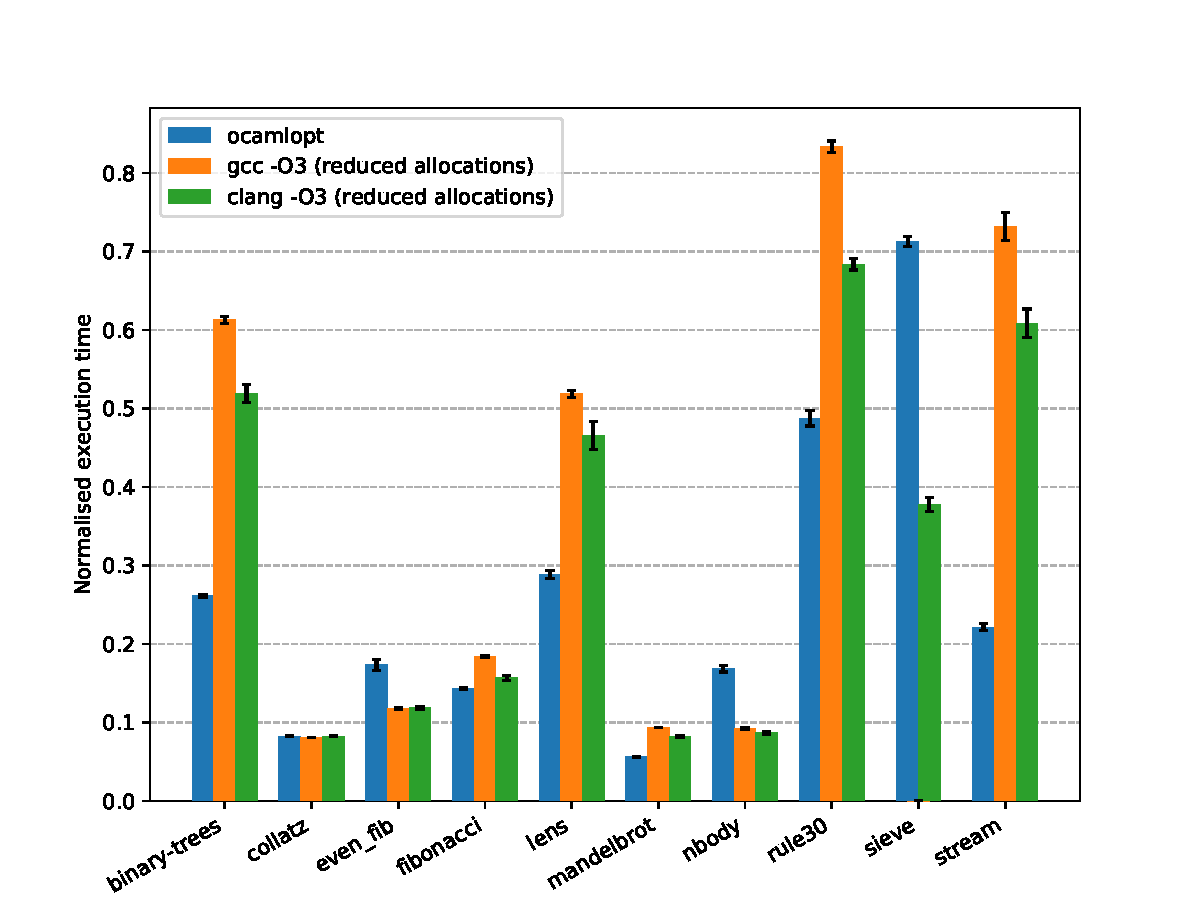
\includegraphics{figs/benchmarks-no-alloc.pdf}
    }

    \caption{Relative speed-up as before in figure~\ref{fig:raw-benchmarks}.
    While most of the benchmarks do not change much, note that the speed-up
    times for \texttt{mandelbrot} and \texttt{nbody} increase signficantly to
    more closely match the native compiler.}

    \label{fig:benchmarks-no-alloc}
\end{figure}

I implemented this mode which is accessible via a C compiler flag, and obtained
results which demonstrated far more favourable execution times especially for
the \texttt{mandelbrot} and \texttt{nbody} benchmarks, as can be seen in
figure~\ref{fig:benchmarks-no-alloc}.

While this change does increase the performance of the compiler, it is worth
noting that this means that polymorphic structures are no longer observable as a
debugger cannot determine all the types at runtime, as well as meaning that
functions that require some degree of runtime reflection such as OCaml's
polymorphic comparisons do not function. This means that while the results
provided by this mode are interesting and represent the performance of the
compiler under perhaps a better representation of polymorphic data, the results
represent an interesting side scenario that is not suitable for use generally.

\section{Stack overflow} \label{stack-overflow}

Curiously, from the benchmark results in figure~\ref{fig:raw-benchmarks}, the
executable produced by GCC under all optimisation levels segfaults for the
benchmark \texttt{sieve}. This is in spite of \texttt{sieve} being written in
tail-recursive style, and \texttt{clang} being able to produce a working
executable.

I therefore performed an investigation using M. Godbolt's compiler
explorer\footnote{\url{https://godbolt.org/}}, and narrowed down the offending
code that causes this to the following: 

\begin{lstlisting}[language=C]
typedef union {
    void* ptr;
} val;

void* g(val);

val f(val x) {
    return {.ptr = g(x)};
}
\end{lstlisting}

When compiled with gcc, this produces the rather confusing output:

\begin{lstlisting}[basicstyle=\ttfamily\footnotesize,
basewidth={.5em,.3em}, frame=single]
0000000000400590 <f>:
  400590:       48 83 ec 08             sub    rsp,0x8
  400594:       e8 57 ff ff ff          call   4004f0 <g>
  400599:       48 83 c4 08             add    rsp,0x8
  40059d:       c3                      ret    
  40059e:       66 90                   xchg   ax,ax
\end{lstlisting}



Somehow, the cast back into the union type prevents \texttt{gcc} from detecting 
the function call is in tail-call position in this specific case, despite the 
fact that the binary representations for the pointer and the union can be the
same and so no conversion would be required in assembler. This causes the
function to compile to a decrement of the stack pointer, a call to another
function, and then an immediate increment of the stack pointer again, when it
would've been equivalent to a \texttt{jmp} instruction to \texttt{g}.


\chapter{Debug sessions} \label{debug-sessions}

\section{The ``sum'' program}

\begin{lstlisting}[language=Caml, numbers=left, stepnumber=1]
external print_int : int -> unit = "print_int"
external newline : unit -> unit = "newline"

let rec foldl f acc = function
  | x :: xs -> foldl f (f acc x) xs
  | [] -> acc

let sum = foldl (+) 0

let a = sum [1; 2; 3]
let _ = print_int a; newline ()
\end{lstlisting}

\section{GDB session of the ``sum'' program} \label{debug-gdb}

\begin{lstlisting}[basicstyle=\linespread{0.8}\ttfamily\footnotesize, basewidth={.5em,.3em}, frame=single, numbers=left, stepnumber=1, breaklines=true, escapechar=]
GNU gdb (Ubuntu 7.11.1-0ubuntu1~16.5) 7.11.1
Copyright (C) 2016 Free Software Foundation, Inc.
License GPLv3+: GNU GPL version 3 or later <http://gnu.org/licenses/gpl.html>
This is free software: you are free to change and redistribute it.
There is NO WARRANTY, to the extent permitted by law.  Type "show copying"
and "show warranty" for details.
This GDB was configured as "x86_64-linux-gnu".
Type "show configuration" for configuration details.
For bug reporting instructions, please see:
<http://www.gnu.org/software/gdb/bugs/>.
Find the GDB manual and other documentation resources online at:
<http://www.gnu.org/software/gdb/documentation/>.
For help, type "help".
Type "apropos word" to search for commands related to "word"...
Reading symbols from test_gdb...done.
(gdb) source ../../../debug/pprint.py
(gdb) break 4
Breakpoint 1 at 0x400fdc: file test.ml, line 4.
(gdb) run
Starting program: /home/tyler/Code/Coursework/observable-ocaml/tests/observability/sum/test_gdb 

Breakpoint 1, local_func_1222 (f_1207=<closure>, acc_1208=0, param_1211=[0: 1 [0: 2 [0: 3 0]]], closure_obj_1221=<closure>) at test.ml:4
4	let rec foldl f acc = function
(gdb) print acc_1208
$1 = 0
(gdb) step
5	  | x :: xs -> foldl f (f acc x) xs
(gdb) print x_1209
$2 = 1
(gdb) print xs_1210
$3 = [0: 2 [0: 3 0]]
(gdb) continue
Continuing.

Breakpoint 1, local_func_1222 (f_1207=<closure>, acc_1208=1, param_1211=[0: 2 [0: 3 0]], closure_obj_1221=<closure>) at test.ml:4
4	let rec foldl f acc = function
(gdb) print acc_1208
$4 = 1
(gdb) step
5	  | x :: xs -> foldl f (f acc x) xs
(gdb) print x_1209
$5 = 2
(gdb) print xs_1210
$6 = [0: 3 0]
(gdb) continue
Continuing.

Breakpoint 1, local_func_1222 (f_1207=<closure>, acc_1208=3, param_1211=[0: 3 0], closure_obj_1221=<closure>) at test.ml:4
4	let rec foldl f acc = function
(gdb) continue
Continuing.

Breakpoint 1, local_func_1222 (f_1207=<closure>, acc_1208=6, param_1211=0, closure_obj_1221=<closure>) at test.ml:4
4	let rec foldl f acc = function
(gdb) step
6	  | [] -> acc
(gdb) p acc_1208
$7 = 6
(gdb) step
main () at test.ml:11
11	let _ = print_int a; newline ()
(gdb) print a_1213
$8 = 6
(gdb) continue
Continuing.
6
[Inferior 1 (process 32184) exited normally]
(gdb) 
\end{lstlisting}

\section{Ocamldebug session of the ``sum'' program} \label{debug-ocaml}

\begin{lstlisting}[basicstyle=\linespread{0.8}\ttfamily\footnotesize, basewidth={.5em,.3em}, frame=single, numbers=left, stepnumber=1, breaklines=true, escapechar=]
	OCaml Debugger version 4.05.0

(ocd) break @ Test_ocaml 4
Loading program... done.
Breakpoint 1 at 106800: file test_ocaml.ml, line 4, characters 15-81
(ocd) run
Time: 24 - pc: 106832 - module Test_ocaml
Breakpoint: 1
5   | x :: xs -> <|b|>foldl f (f acc x) xs
(ocd) print acc
acc: 'a = <poly>
(ocd) print x
x: 'a = <poly>
(ocd) print xs
xs: 'a list = [<poly>; <poly>]
(ocd) run
Time: 26 - pc: 106832 - module Test_ocaml
Breakpoint: 1
5   | x :: xs -> <|b|>foldl f (f acc x) xs
(ocd) print x
x: 'a = <poly>
(ocd) print xs
xs: 'a list = [<poly>]
(ocd) run
Time: 28 - pc: 106832 - module Test_ocaml
Breakpoint: 1
5   | x :: xs -> <|b|>foldl f (f acc x) xs
(ocd) run
Time: 30 - pc: 106864 - module Test_ocaml
Breakpoint: 1
6   | [] -> <|b|>acc
(ocd) print acc
acc: 'a = <poly>
(ocd) step
Time: 31 - pc: 107040 - module Test_ocaml
10 let a = sum [1; 2; 3]<|a|>
(ocd) next
Time: 47 - pc: 107052 - module Test_ocaml
11 let _ = print_int a<|a|>; newline ()
(ocd) print a
a: int = 6
(ocd) run
6
Time: 79
Program exit.
(ocd)
\end{lstlisting}

\chapter{Project Proposal}

\section*{Introduction and Description of the Work}

This project involves the implementation of a compiler from OCaml to C in such
a way that will allow the resulting executable to be compatible with
DWARF-based debugging tools, such as \texttt{gdb}. This project will use the
existing front-end of the OCaml compiler, but implement a very different
back-end which outputs valid C code that can be compiled using a tool such as
\texttt{gcc} into a debuggable executable. The focus of the compiler is to
optimise for debuggability, or ``observability'', by taking advantage of the
numerous debugging tools available of the C compilation toolchain.

Since the implementation of the full OCaml language is likely too ambitious for
one project, the core project will instead revolve around the implementation of
an interesting subset of OCaml which still provides technically interesting
challenges in its implementation, while extension tasks may extend the
implementation to cover a wider subset of the entire language. An informal
description of said subset will be given in the Substance and Structure
section.

The ``observability'' of the compiler means that where possible the debugger
should behave \emph{as if} it was debugging the OCaml code. This means that the
debugger should consider sections of the compiled machine code to be mapped to
the appropriate lines of code in OCaml. Furthermore, locally bound variables
should be visible from the debugger when execution has reached the relevant
point, meaning that local variables in the C code should mirror the variables
in the OCaml code.

In addition, features such as closures and parametric polymorphism must be
implemented carefully since these features don't have any similar structures in
C for which they could've been mapped to, but also to maintain
``observability'' these must be ``transparent'' to the debugger (for example, a
polymorphic function of the type \verb!'a -> 'a! that has been instantiated as
the type \verb!int -> int! should have this quality be visible from the
debugger). These qualities can be implemented using user-defined commands for
\texttt{gdb}.

The resulting compiler can be evaluated in mainly two contexts. One of these is
a straightforward performance comparison, where a testbed of OCaml programs are
benchmarked across the OCaml native compiler, the OCaml bytecode compiler, and
this project. The other context is the ``observability'' of the compiler; where
programs are stopped at a certain point of their execution and inspected, to
see how much of the internal state of the stack is recoverable. This can be
made in comparison with OCaml's bytecode debugger, \texttt{ocamldebug}.

\section*{Resources Required}

No special resouces are requred that are not open source and freely available
for download.

\section*{Starting Point}

The project, at least initially, will be a fork of the OCaml compiler
obtainable at \url{github.com/ocaml/ocaml} which will take the same front-end
as the existing compiler, but will implement a new back-end for compilation
into C. The work may use other libraries such as \texttt{libffi} and
\texttt{liballocs} but no work of similar scope to the project.

\section*{Substance and Structure of the Project}

The core of the project will be devoted into the implementation of three
incrementally expanding subsets of OCaml. These subsets have been identified
such that each is sufficient to write nontrivial programs in, and features have
been grouped by relation to each other. In this manner work can be easily split
into 3 discrete blocks, each of which will support a new collection of
programs by their completion.

\subsection*{Subset 1}

Subset 1 will be a very simple language with only a limited number of types and
language constructs. The subset will contain only the basic boolean, integer,
floating point and \texttt{unit} types, basic string support (for
input/output), top level function declarations with \texttt{let} and
\texttt{let rec}, which only accept one argument (so as to sidestep the problem
of partial application and closures), \texttt{if}, \texttt{for},
\texttt{while}, \texttt{ref}, as well as basic arithmetic and boolean
operations.

These features were chosen because because they very easily make for a small
minimalist language, and all constructs more or less have direct analogues in C
meaning translation from AST to C code should be fairly easy. Nonetheless, this
small subset is sufficient to write simple programs.

\subsection*{Subset 2}

Subset 2 will focus on the implementation of types and polymorphism, and will
support tuples, lists, parametric polymorphism, algebraic data types, record
types, and \texttt{match} expressions.

The implementation of this subset will require the design of an object
representation for OCaml values. Tuples and record types map easily to structs
in C, while a tagged union can be used for OCaml's ``sum of products'' approach
to algebraic data types. On the first pass, it is quite likely that a naive
``tagged pointer'' type will be used for support for polymorphism, but
extension tasks may experiment with eliminating this need via some method.

The addition of algebraic data types greatly increases the scope of supported
programs, and allows for functions taking multiple arguments (via tuples), list
processing functions, and more complex data structures such as binary trees.

\subsection*{Subset 3}

Subset 3 will finally add treatment of functions as first-class values. This
will include lambdas, lexical closures, and partial application of functions.

The implementation of this subset will require some representation of closures.
While C does support function pointers, it has no lexical closures and as such
a representation where closures are function pointers with an extra
\texttt{void *} pointer that refers to data in the closure is likely to be the
implementation on the first pass. As an extension task, more performant ways of
implementing closures may be investigated, such as potentially dynamically
generating entry points that push the required arguments before jumping to the
body of the function. 

The addition of these features will make higher-order functions representable,
and make available functions such as \texttt{map}, \texttt{filter}, function
composition etc. At this point subset 3 can be considered a fairly minimal but
full-featured functional language.

\subsection*{Evaluation}

Evaluation will require the creation of a small library of test programs. These
programs should be novel and exhibit the full range of language features
supported by the subsets.

Two main methods will then be used to evaluate the compiler. One is
benchmarking performance of the test programs with the existing OCaml native
compiler and the OCaml bytecode compiler. While it is not expected that the C
compiler will match the performance of OCaml official compilers, the goal is to
be within a reasonable margin so that the performance of compiled C code is
comparable. The performance evaluation will be a simple measurement of the
runtime of the compiled executable in relation to the running time of the
executable produced by the OCaml native compiler and the running time of the
interpreter on the bytecode produced by the OCaml bytecode compiler. The test
suite for the performance evaluation will have to be partly written as part of
the project, and partly adapted from the existing OCaml compiler test suite
(\url{github.com/ocaml/ocaml/tree/trunk/testsuite}) or possibly the Computer
Language Benchmarks Game (\url{benchmarksgame.alioth.debian.org}). Since the
compilation source is only a subset of OCaml, not all of the existing test
suite programs will be relevant, and others will require some adaptation for
them to work for the project.

The other method will be the evaluation of the ``observability'' of the C code.
This will take place in two parts: firstly, we can do a test for
``observability'': this will entail a minimum list of requirements, such as
ability to step through OCaml code, ability to print locally bound values,
ability to print types of locally bound variables, and ability to show
instantiation of polymorphic functions into specific types. The second is to
compare the debug outputs of the C code and the OCaml code. The native OCaml
compiler does not allow observation of locally bound values at all, so our C
compiler should beat this easily; although a more interesting comparison would
be with the OCaml bytecode debugger. Breakpoints could be set at randomly
chosen call sites, and the stack traces, visible locals etc.\ could be compared
between \texttt{ocamldebug} and the debug output of the C code.

\subsection*{Extension Tasks}

This project leaves a lot of room for extension tasks. An obvious extension is
to extend the subset to be a more complete subset of OCaml. The next steps
taken would likely be module and exception support, although both are far more
complex features to attempt for implementation in C.

More realistic extension tasks would be changes to the existing code in order
to make it more performant. This would involve improvements to the
implementation of polymorphic functions and closures, as described in their
respective sections prior.

Another plausible extension task is to improve the debug output of OCaml
values. Since C does not have an exact analogue for all OCaml values the debug
output from \texttt{gdb} for example will not look exactly like their OCaml
representation. However, \texttt{gdb} supports the use of custom formatters
written in Python for types and a task to implement a way to generate
formatters to print OCaml values correctly is a suitable extension task.

\section*{Success Criteria}

The following criteria should be achieved at the completion of the project:

\begin{itemize}

    \item A working compiler, that is able to compile the language as described
        in Subset 3 into C code correctly;

    \item An evaluation of performance between the output of the compiler and
        the OCaml native and bytecode compilers;

    \item An evaluation of ``observability'' in the compiled executable with
        tools such as \texttt{gdb}. 

        The evaluation should focus on the following:

        \begin{itemize}

            \item Ability to set breakpoints and step through the compiled
                executable as if it was OCaml code;

            \item Ability to view locally bound variables, and their types,
                although perhaps only as a C ``version'' of the resulting data;

            \item Ability to print more complex data structures, such as ADTs,
                record types and lists;

            \item Similar and comparable output between the debug output and
                the same code running in \texttt{ocamldebug}.

        \end{itemize}

\end{itemize}

Further success criteria, which are not expected to be achieved through the
core project, but interesting as extension tasks may be:

\begin{itemize}

    \item Ability to view the instantiated types of polymorphic functions;

    \item Ability to view data formatted as OCaml values, using specially
        written formatters for \texttt{gdb};

    \item Any number of optimisations on the generated code, resulting in
        better performance benchmarks.

\end{itemize}

\section*{Timetable and Milestones}

\subsection*{20 October --- 3 November}

Initial experiments and reading. Familiarise with the OCaml compiler source
code and obtain typed AST\@. Set up development environment. Write testbed of
evaluation programs so that features can be tested and evaluated immediately
after their implementation.

Milestones: A completed small library of OCaml programs, plus a way of
obtaining the typed AST from the OCaml compiler.

\subsection*{4 November --- 17 November}

Implementation of Subset 1. Evaluation of Subset 1 performance with respect to
the OCaml native and bytecode compilers.

Milestones: A collection of programs now compileable by the Subset 1 compiler,
along with their running times collected in comparison with the OCaml
compilers.

\subsection*{18 November --- 15 December}

Implementation of Subset 2. This is expected to take longer than the
implementation of Subset 1 to take into account that special care needs to be
taken when designing object representations of OCaml values and implementation
of parametric polymorphism. Evaluation of Subset 2 performance with respect to
OCaml compilers.

Milestones: A larger collection of programs now compileable by the Subset 2
compiler, along with their performance results in comparison with the OCaml
compilers.

\subsection*{16 December --- 29 December}

(Two week break for Christmas)

\subsection*{30 December --- 12 January}

Implementation of Subset 3. Evaluation of Subset 3 performance, as well as
comparison between the debug output of the compiled code with
\texttt{ocamldebug}.

Milestones: Completion of core project with the implementation of Subset 3.
Some evaluation results (although perhaps not complete) for the core project.

\subsection*{13 January --- 26 January}

Write up of the Progress Report. Perform any new evaluation tasks that were
missed but become apparent in the write up of the Progress Report. Review the
remainder of the project in context with the existing work and determine which
extension tasks are best to pursue.

Milestones: Completed core project with evaluation, with a completed Progress
Report ready for submission. Entire project reviewed with supervisor and
overseers.

\subsection*{27 January --- 9 February}

Submission of Progress Report. Revise evaluation tasks with feedback from
Progress Report. Prepare Progress Report presentation.

\subsection*{10 February --- 23 February}

Start work on dissertation, as well as the implementation of ways of making the
compiled code more performant. Investigation and use of perhaps \texttt{libffi}
and \texttt{liballocs} to improve performance and observability.

Milestones: The introduction and preparation sections of the dissertation
complete. Improvements on the compiler made, with evaluation results to show
improvements in performance of the compiled output.

\subsection*{24 February --- 9 March}

Start writing the implementation section of dissertation. Implementation of the
generation of custom formatters for \texttt{gdb}, which will make the debug
output easier to read and interpret as OCaml values.

Milestones: Implementation section of the dissertation at least half complete.
Improvements to debug output of debuggers run on the compiled executables.

\subsection*{10 March --- 22 March}

Finish writing implementation section of dissertation. Start evaluation
section. Pick up any further evaluation tasks at this point that become
apparent.

Milestones: Finished implementation section, evaluation section at least half
complete. Revised evaluation tasks in accordance with the write up of the
evaluation section.

\subsection*{23 March --- 5 April}

Finish evaluation and conclusion sections of the dissertation. Deliver draft
dissertation to supervisor and director of studies for feedback. Spend time
working on whatever is in greatest need of attention.

Milestones: Submit a complete draft of the dissertation for review to
supervisor and director of studies.

\subsection*{6 April --- 19 April}

Revise dissertation based on feedback received. Finish any last tasks that
require performing, which are hopefully minor at this point in time. Send
revised drafts for further rounds of review.

\subsection*{20 April ---}

Final adjustments and revisions to dissertation and the body of code. Prepare
for submission of dissertation.

Milestone: Submission of dissertation.

\newpage

\section*{Resource Declaration}

No special resources are required for this project other than those that are
not already available as open source code.



\end{document}
